\documentclass[a4paper, 14pt, oneside]{Thesis}
\usepackage{ulem}
\usepackage[square, numbers, comma, sort&compress]{natbib}  % Use the "Natbib" style for the references in the Bibliography
\usepackage{verbatim} 
\usepackage{pslatex} %To set the font as Times New Roman
\usepackage{amsbsy} 
\usepackage{amsfonts}
\usepackage{graphicx}
\usepackage{array}
\usepackage{dcolumn}
\usepackage{amsmath}
\usepackage{latexsym}
\usepackage{amssymb}
\usepackage{epsfig}
\usepackage{verbatim} 
\usepackage{epsfig,graphics}
\usepackage{subfigure}
\usepackage{tikz}
\usepackage{float}
\usepackage{algorithm}
\usepackage{algpseudocode}
\usepackage{subcaption}
\usepackage{placeins}  % For FloatBarrier

\makeatletter
\numberwithin{algorithm}{chapter}
\renewcommand\section{\@startsection {section}{1}{\z@}%
                                   {-3.5ex \@plus -1ex \@minus -.2ex}%
                                   {2.3ex \@plus.2ex}%
                                   {\normalfont\Large\bfseries\raggedright}}
\renewcommand\subsection{\@startsection{subsection}{2}{\z@}%
                                     {-3.25ex\@plus -1ex \@minus -.2ex}%
                                     {1.5ex \@plus .2ex}%
                                     {\normalfont\large\bfseries\raggedright}}
\makeatother

%\usepackage{fancyhdr}
%\usepackage{lipsum}

%To have 1. instead of [1] in the bibliographic entry
\makeatletter
\renewcommand\@biblabel[1]{#1.}
\makeatother

% To remove hyphenation
\tolerance=1
\emergencystretch=\maxdimen
\hyphenpenalty=10000
\hbadness=10000
%
%----To make sure the page numbers are in the top middle of each page.
\fancypagestyle{Thesis}{
\fancyhf{}
\fancyhead[C]{\thepage}
\%lfoot{\thepage}
\pagestyle{fancy}
}
%redefine the plain pagestyle
%\fancypagestyle{plain}{
%\fancyhf{}
%\fancyhead[C]{\thepage}
%}
%----------------------------------------------------------------------
%% ------------------------s----------------------------------------
% Some new environments for the paper
%
\newtheorem{dfn}{Definition}[section]
\newtheorem{prop}[dfn]{Proposition}
\newtheorem{lem}[dfn]{Lemma}
\newtheorem{thm}[dfn]{Theorem}
\newtheorem{cor}[dfn]{Corollary}
\newtheorem{clm}[dfn]{Claim}
\newtheorem{fact}[dfn]{Fact}
%
%\newcommand{\RightBox}{\begin{flushright} $\Box$ \end{flushright}}
\newcommand{\RightBox}{{\phantom{a}}\hfill $\Box$ \\}
%\newenvironment{proof}{{\bf Proof:~}}{\RightBox}
\newenvironment{prf}{{\bf Proof~Idea:~}}{\RightBox}
%\newcommand{\claim}[1]{{\bf Claim #1:~}}
%
\newcommand{\Dfn}[1]{Definition \ref{dfn:#1}}
\newcommand{\Prop}[1]{Proposition \ref{prop:#1}}
\newcommand{\Lem}[1]{Lemma \ref{lem:#1}}
\newcommand{\Thm}[1]{Theorem \ref{thm:#1}}
\newcommand{\Cor}[1]{Corollary \ref{cor:#1}}

%Action-indexed diamond modality
\newcommand{\Adiam}[1]{\mbox{$\langle #1 \rangle$}}
\newcommand{\diamin}{\Diamond\kern-0.5em{\raisebox{.25ex}{\rm -}}\kern0.175em}
\newcommand{\until}{\mbox{\large\bf U}}
\newcommand{\since}{\mbox{\large\bf S}}
\newcommand{\nxt}{\mbox{$\bigcirc$}}
\newcommand{\nxtdot}{\displaystyle \bigodot}
\newcommand{\past}{\diamin}
\newcommand{\ifpast}{\mbox{$\boxminus$}}
\newcommand{\now}{\mbox{$\langle now \rangle$}}
\newcommand{\Now}{\mbox{$[now]$}}
\newcommand{\pres}{\mbox{$\rangle \langle$}}
\newcommand{\snd}{\mbox{\large\bf s}}
\newcommand{\rec}{\mbox{\large\bf r}}
\newcommand{\nc}{\mathbf{no\_comm}}

%Propositional connectives
%\newcommand{\implies}{{\raisebox{.20ex}{$\scriptstyle ~\supset~$}}}
\newcommand{\Not}{\mbox{$\lnot$}}
\newcommand{\xor}{\oplus}
\newcommand{\True}{\mathit{True}}
\newcommand{\False}{\mathit{False}}
\newcommand{\Imply}{\supset}
%Large symbols
\newcommand{\andover}{\displaystyle \bigwedge}
\newcommand{\orover}{\displaystyle \bigvee}
\newcommand{\capover}{\displaystyle \bigcap}
\newcommand{\cupover}{\displaystyle \bigcup}
\newcommand{\piover}{\displaystyle \Pi}
\newcommand{\ohat}[1]{\widehat{#1}}
\newcommand{\otilde}[1]{\widetilde{#1}}
\newcommand{\obar}[1]{\overline{#1}}
\newcommand{\Sigtil}{\mbox{$\otilde{\Sigma}$}}
\newcommand{\DA}{\mbox{$\Sigtil~=~(\Sigma_1, \dots, \Sigma_n)$}}

%Useful symbols
\newcommand{\derives}{\vdash}
\newcommand{\defn}{\mbox{$~\stackrel{\rm def}{=}~$}}
\newcommand{\qneq}{\mbox{$~\stackrel{\rm ?}{=}~$}}
\newcommand{\eqv}{\approx}
\newcommand{\hash}{\sharp}
\newcommand{\restr}{\lceil}
%\newcommand{\bot}{\bottom}
\newcommand{\nat}{{\bf N}}
\newcommand{\pfin}[1]{\mbox{$\wp_{fin}(#1)$}}
%\newcommand{\mod}[1]{\mbox{$|#1|$}}
\newcommand{\memb}[2]{\mbox{${#1} \in {#2}$}}
\newcommand{\E}{\mathbf{E}}



%Some roman words in math mode
\newcommand{\Iff}{\mbox{~iff~}}
\newcommand{\Where}{\mbox{~where~}}
%\newcommand{\And}{\mbox{~and~}}
\newcommand{\Implies}{\mbox{~implies~}}

%Relations

% structures
\newcommand{\Sigstr}{\mbox{$\Sigma^*$}}
\newcommand{\TS}{\mbox{$TS = (Q,\to)$}}  %generates TS=(Q,->)
\newcommand{\TSP}{\mbox{$TS = (Q,\To)$}}         %generates TS=(Q,=>)
\newcommand{\TSi}{\mbox{$TS_i = (Q_i,\to_i)$}}           
\newcommand{\TSE}{\mbox{$TS_{ES}$}}
\newcommand{\TSN}{\mbox{$TS_{\cal N}$}}
\newcommand{\ES}{\mbox{$ES = (E,\leq,\#)$}}       %generates ES=(E,<=,#)
\newcommand{\LES}{\mbox{$ES = (E,\leq,\#,\phi)$}} %generates ES=(E,<=,#,phi)
\newcommand{\Tmdl}{\mbox{$M = (TS,V)$}}          %generates M = (TS,V)
\newcommand{\cfin}[1]{\mbox{$C_{#1}$}}           %finite configurations of
\newcommand{\fincon}[1]{\mbox{$C_{#1}^{fin}$}}  %finite configurations

% classes
\newcommand{\mdl}[1]{\mbox{${\cal M}_{#1}$}}%generates script M with subscript
\newcommand{\dmodels}{\mbox{$\models_{Det}~$}}

% For transitions steps
\newcommand{\step}[1]{\mbox{$\stackrel{#1}{\to}$}}
\newcommand{\Funnyto}{\rightsquigarrow}
\newcommand{\longstep}[1]{\mbox{$\stackrel{#1}{\longrightarrow}$}}
\newcommand{\emptystep}{\step{\emptyset}}
\newcommand{\reach}[1]{\mbox{${\cal R}(#1)$}}
\newcommand{\reachin}[2]{\mbox{${\cal R}_{#1}(#2)$}}

% For a "double-lined" transition relation
\newcommand{\To}{\Rightarrow}
\newcommand{\From}{\Leftarrow}
\newcommand{\Step}[1]{\mbox{$\stackrel{#1}{\To}$}}
\newcommand{\Longstep}[1]{\mbox{$\stackrel{#1}{\Longrightarrow}$}}
\newcommand{\Longlongstep}[1]{\mbox{$\stackrel{#1}{\Longlongrightarrow}$}}
\newcommand{\Emptystep}{\Step{\emptyset}}

% Net theory
\newcommand{\presca}[1]{\mbox{${ }^{\bullet}#1$}}
\newcommand{\postsca}[1]{\mbox{$#1 \, { }^{\bullet}$}}%

%The built in downarrow generates too much space after it
%\newcommand{\down}{\mbox{$\downarrow \!$}}
\newcommand{\down}{\mbox{$\downarrow$}}
\newcommand{\up}{\mbox{$\uparrow \!$}}
\newcommand{\ldot}{{\rm <}\kern-0.37em{\raisebox{.25ex}{\bf .}}\kern0.375em}

%Trace theory
\newcommand{\edoti}{\mbox{$\doteq_I$}}
\newcommand{\eqi}{\mbox{$=_I$}}
\newcommand{\edotk}{\mbox{$\doteq_k$}}
\newcommand{\eqk}{\mbox{$=_k$}}

\newcommand{\calL}{\mathcal{L}}
\newcommand{\calB}{\mathcal{B}}
\newcommand{\posetlang}[1]{\mbox{${\calL}^{po}(#1)$}}%poset language of an SCA
\newcommand{\bddlang}[2]{\mbox{${{\calL}^{#1}}(#2)$}} %bounded buffer language

\newcommand{\calS}{\mathcal{S}}
\newcommand{\calA}{\mathcal{A}}
\newcommand{\calC}{\mathcal{C}}
\newcommand{\calE}{\mathcal{E}}
\newcommand{\calG}{\mathcal{G}}



\newcommand{\calQ}{\mathcal{Q}}
\newcommand{\calD}{\mathcal{D}}
\newcommand{\calCN}{\mathcal{CN}}
\newcommand{\calI}{\mathcal{I}}
\newcommand{\calF}{\mathcal{F}}
\newcommand{\calM}{\mathcal{M}}

\begin{document}

\frontmatter	  % Begin Roman style (i, ii, iii, iv...) page numbering


%  Title Page

\title{Reasoning Failure Boundaries in ECG Foundation Models Under Progressive Physiological Information Loss}
\authors{\texorpdfstring{
    \begin{tabular}{@{}l@{\hspace{0.4in}}l@{}}
        VIJAY K & 3122235001157 \\
        SIDDHARTH CHANDRASEKAR S & 3122235001310 \\
        VEDANTH M S & 3122235001314
    \end{tabular}
}{VIJAY K (3122235001157), SIDDHARTH CHANDRASEKAR S (3122235001310), VEDANTH M S (3122235001314)}}
\addresses  {\\\Computer Science \& Engineering\\}
\date       {\large {October 2026}}

\maketitle
%% ----------------------------------------------------------------

\setstretch{1.3}
\fancyhead{}  % Clears all page headers and footers
\rhead{\thepage}  % Sets the right side header to show the page number
\lhead{}  % Clears the left side page header

\pagestyle{fancy}  % Finally, use the "fancy" page style to implement the FancyHdr headers


\Declaration{ 
%
\quad Certified that this project report titled \textbf{``REASONING FAILURE BOUNDARIES IN ECG FOUNDATION MODELS UNDER PROGRESSIVE PHYSIOLOGICAL INFORMATION LOSS''} is the \textit{bonafide} work of \textbf{Vijay K (3122235001157)}, \textbf{Siddharth Chandrasekar S (3122235001310)}, and \textbf{Vedanth M S (3122235001314)} who carried out the project work under my supervision.
\\
Certified further that to the best of my knowledge the work reported herein does not form part of any other thesis or dissertation on the basis of which a degree or award was conferred on an earlier occasion on this or any other candidate. \\
  \newlength{\aulength} 
  \settowidth{\aulength}{SSN College of Engineering,}
  \newlength{\auclength} 
  \settowidth{\auclength}{(HEAD OF THE DEPARTMENT)}

\begin{flushleft}
\begin{minipage}[t]{0.45\linewidth}
    \textbf{Dr. T.T. MIRNALINEE}\\
    \textbf{HEAD OF THE DEPARTMENT}\\
    Professor\\
    Department of CSE\\
    SSN College of Engineering\\[6pt]
    Kalavakkam - 603 110
\end{minipage}
\hfill 
\begin{minipage}[t]{0.45\linewidth}
    \textbf{Dr. ANUSHA JAYASIMHAN}\\
    \textbf{SUPERVISOR}\\
    Associate Professor\\
    Department of CSE\\
    SSN College of Engineering\\[6pt]
    Kalavakkam - 603 110
\end{minipage}
\end{flushleft}


\medskip
Submitted for project viva-voce examination held on\ldots\ldots\ldots\ldots
\\
\\
\\
{\bf EXTERNAL EXAMINER}\hfill
{\bf INTERNAL EXAMINER}
}
\clearpage
%% Abstract in Tamil

% Acknowledgement
%\setstretch{1.3}

\clearpage
%% ----------------------------------------------------------------

% The Abstract Page

\acknowledgements{
We thank GOD, the almighty for giving us strength and knowledge to do this project.

We would like to express our deep sense of gratitude to our guide \textbf{Dr. ANUSHA JAYASIMHAN}, Associate Professor, Department of Computer Science and Engineering, for her valuable advice and suggestions as well as her continued guidance, patience and support that helped us to shape and refine our work.

Our sincere thanks to  \textbf{Dr. T.T. MIRNALINEE}, Professor and Head of the Department of Computer Science and Engineering, for her words of advice and encouragement. We would like to thank \textbf{Dr. SURESH JAGANATHAN}, Project Coordinator, and our project panel members for their valuable suggestions throughout this project.

 We also express our appreciation to \textbf{Dr. S. RADHA}, Principal, for all the help she has rendered during this course of study.

 We would like to extend our sincere thanks to all the teaching and non-teaching staff of our department who have contributed directly and indirectly during the course of our project work.
Finally, we would like to thank our parents and friends for their patience, cooperation and moral support throughout our life.
\newline
\newline
\newline
\newline
{\bf VIJAY K}\hfill
{\bf SIDDHARTH CHANDRASEKAR S}\hfill 
{\bf VEDANTH M S}
\clearpage  % Abstract ended, start a new page

\addtotoc{ABSTRACT} % Add the "Abstract" page entry to the Contents
\abstract{ \begin{spacing}{1.5}
ECG foundation models are increasingly used for automated interpretation, yet a model may still give a confident diagnosis when some leads are missing and the evidence for that diagnosis was never recorded. This project studies how ECG model behaviour changes under progressive lead removal. Recordings from PTB-XL, Chapman-Shaoxing and MIMIC-IV-ECG were standardised and masked at seven lead-availability levels (12, 10, 8, 6, 4, 2 and 1 leads) without reconstructing the missing signals. A frozen ECG-FM encoder produced representations, and a Control Reasoning Transformer combined them with rule-based observations and the lead mask to classify eight conditions. On the test partition, macro-AUROC stayed between 0.9479 and 0.9540 down to two leads and fell to 0.9215 with lead II alone, and a 4-lead configuration containing V1 outperformed the 6-lead limb configuration; these are descriptive results from one seed of an authorisation-unverified evaluation. A grounding gate with SUPPORTED, CONTRADICTED and UNAVAILABLE evidence states and the Reasoning Failure Boundary are specified but not yet implemented, and a SNOMED CT-based Clinical Knowledge Prior is planned future work.

\par\noindent\textbf{Keywords:} Electrocardiogram; Foundation models; Lead removal; Evidence grounding; Reasoning failure boundary
\end{spacing}
}
\clearpage
%%% DUMMY PAGE FOR TAMIL ABSTRACT WHICH WILL BE PRINTED SEPARATELY
%%% Since LaTeX can't print tamil characters, you've to type tamil 
%%% abstract in some other editors and print it separately. When
%%% binding the thesis place the tamil abstract in place of this blank page
%%% I'm adding this blank page for Table of Contents to point to the right page

%\pagestyle{empty}
%\newpage
%\mbox{}
%\clearpage

\pagestyle{plain}  %The page style headers have been "empty" all this time, now use the "fancy" headers as defined before to bring them back

%% ----------------------------------------------------------------
\lhead{\emph{Contents}}  % Set the left side page header to "Contents"

\tableofcontents % Write out the Table of Contents


%% ----------------------------------------------------------------
\lhead{\emph{List of Tables}}  % Set the left side page header to "List of Tables"
%\begin{spacing}{4}
%\hspace{2.5in} \textbf{List of Tables} \par 
\listoftables
%\end{spacing}

%% ----------------------------------------------------------------
\lhead{\emph{List of Figures}}  % Set the left side page header to "List if Figures"
\listoffigures  % Write out the List of Figures


%2.1 LITERATURE SURVEY OF METAMORPHIC TESTING. . . . . . . . . . . .  13


 % Write out the List of Tables


\mainmatter	  % Begin normal, numeric (1,2,3...) page numbering
\pagestyle{myheadings}  % Return the page headers back to the "fancy" style

\begin{spacing}{1.5}
\chapter{INTRODUCTION}

The electrocardiogram (ECG) is a non-invasive recording of the electrical activity of the heart, measured as potential differences between electrodes placed on the limbs and the chest. The standard 12-lead ECG combines limb leads and precordial leads to observe cardiac electrical activity from several directions, and it remains the reference recording for assessing rhythm, conduction and myocardial injury \cite{KLIGFIELD2007AHA}. Many diagnostic findings are tied to particular leads, and the AHA/ACCF/HRS recommendations set out separate criteria for intraventricular conduction disturbances, such as bundle branch block, and for acute ischaemia and infarction \cite{SURAWICZ2009AHA,WAGNER2009AHA}. The diagnostic value of an ECG therefore depends on which leads were recorded.

Automated interpretation of the ECG has developed from rule-based measurement programs \cite{SCHLAPFER2017COMPUTER} into deep neural networks trained on large clinical databases \cite{HANNUN2019CARDIOLOGIST,STRODTHOFF2021PTBXL}. More recently, ECG foundation models have been pretrained on very large collections of unlabelled recordings using self-supervised objectives, so that a single pretrained encoder can provide general-purpose signal representations for many downstream tasks \cite{MCKEEN2025ECGFM}. In practice, however, a complete 12-lead recording is not always available. Smaller and easier-to-use recording devices often capture only a subset of the leads, and single-lead ambulatory monitors are already in clinical use \cite{HANNUN2019CARDIOLOGIST,REYNA2022ISSUES}. When leads are missing, a model may still produce a confident diagnosis, but the physiological evidence that a clinician would require for that diagnosis may no longer be present in the signal.

This project, titled Reasoning Failure Boundaries in ECG Foundation Models Under Progressive Physiological Information Loss, studies this situation in a controlled manner. ECG recordings from three public cohorts, PTB-XL, Chapman-Shaoxing and MIMIC-IV-ECG, are standardised to a common format and evaluated on eight conditions: normal ECG, atrial fibrillation, right and left bundle branch block, sinus bradycardia, sinus tachycardia, first-degree atrioventricular block and myocardial infarction. Each recording is presented at seven lead-availability levels of 12, 10, 8, 6, 4, 2 and 1 leads. Missing leads are set to zero and are never reconstructed, so that the model only receives information that was actually recorded. A publicly released ECG foundation model, ECG-FM, is used as a frozen encoder that converts each degraded recording into a 768-dimensional representation \cite{MCKEEN2025ECGFM}.

On top of this encoder, the project builds a reasoning stage that combines the learned representation with rule-based measurements extracted only from the available leads. A Control Reasoning Transformer, which uses no external clinical knowledge, has been implemented and trained during the first half of the project. It produces probabilities for the eight conditions together with an attention-based reasoning trace. The project further proposes a deterministic grounding gate that labels each clinical claim as supported, contradicted or unavailable, and a knowledge-augmented reasoning path based on a Clinical Knowledge Prior derived from SNOMED CT. Both of these components have been specified but not yet implemented, and they are treated in this report as planned work.

\section{MOTIVATION}
The ECG is a quick and non-invasive cardiac investigation that is informative across a broad range of rhythm, conduction and ischaemic conditions \cite{KLIGFIELD2007AHA}. Its interpretation relies on measurements derived from the waveform, which lead to standardised diagnostic statements \cite{KLIGFIELD2007AHA}. Because these criteria refer to specific leads and measurements, an interpretation can in principle be checked against the recording from which it was made.

Automated ECG interpretation has a long history, and a review of computer-interpreted ECGs notes that the majority of the millions of ECGs recorded each year are analysed automatically, that limitations in diagnostic accuracy have persisted, and that clinicians may accept computer statements without verifying them \cite{SCHLAPFER2017COMPUTER}. Deep learning has since improved classification performance substantially on large datasets \cite{HANNUN2019CARDIOLOGIST,STRODTHOFF2021PTBXL}. As performance improves, it becomes more important to understand what evidence an automated system uses before its output is relied upon.

Foundation models extend this development by learning representations from unlabelled data that can be reused across tasks \cite{MCKEEN2025ECGFM}. ECG-FM, the model used in this project, follows the wav2vec 2.0 architecture and was pretrained with a combination of masked prediction, contrastive multi-segment coding and random lead masking \cite{MCKEEN2025ECGFM,OH2022LEADAGNOSTIC}. Random lead masking is intended to make a model usable when only some leads are present, but this raises a question that accuracy alone cannot answer: whether a diagnosis produced after leads are removed is still justified by the remaining signal.

Reduced-lead recordings are common in practice. Smaller and lower-cost devices that record fewer leads may widen access to cardiac care, although their diagnostic potential is not yet clear \cite{REYNA2022ISSUES}, and single-lead ambulatory monitors are already used for rhythm assessment \cite{HANNUN2019CARDIOLOGIST}. Research on reduced-lead classification has shown that for some tasks a limited set of leads can retain much of the classification performance of the full 12-lead ECG \cite{REYNA2022ISSUES,LAI2021LEADSELECTION}. Preserved classification performance, however, does not imply that the specific evidence for each diagnosis is still observable.

Progressive lead removal provides a controlled way to study this question. Because every recording is evaluated at each of the seven availability levels, any change in the model's behaviour can be attributed to the removed leads rather than to differences between patients. Missing leads are not reconstructed from the remaining ones. Reconstructed leads would be estimates rather than measurements \cite{PRESACAN2025RECON}. Masking without reconstruction keeps a clear distinction between information that was recorded and information that was not.

A further motivation concerns explanations. Current explanation methods are unlikely to provide reliable explanations for individual patients \cite{GHASSEMI2021FALSEHOPE}, and attention weights in particular cannot be assumed to explain a model's decision \cite{JAIN2019ATTENTION}. A useful explanation of an ECG diagnosis should therefore be checked against measurable evidence, and the check must separate three situations: the evidence is present and agrees with the claim, the evidence is present and disagrees with it, or the evidence cannot be assessed because the required leads are absent. This need to identify where model claims stop being supported by the available leads is the motivation for investigating Reasoning Failure Boundaries in ECG foundation models.

\section{BACKGROUND}
The standard 12-lead ECG is recorded from ten electrodes. Electrodes on the right arm, left arm and left leg form the limb leads I, II and III, the right-leg electrode serves as a reference, and six chest electrodes form the precordial leads V1 to V6. The augmented limb leads aVR, aVL and aVF are computed from the same limb electrodes \cite{KLIGFIELD2007AHA}. Consequently, lead III and the three augmented leads can be expressed as linear combinations of leads I and II, whereas the six precordial leads carry information that cannot be obtained from the limb leads. This relationship is important for the present work, since removing a derived limb lead does not remove electrical information that is available from leads I and II, whereas removing precordial leads does.

Different leads observe the heart from different directions, and diagnostic criteria are defined with respect to these views. The limb leads describe activity in the frontal plane, while the precordial leads describe activity in the horizontal plane. Separate parts of the AHA/ACCF/HRS recommendations address intraventricular conduction disturbances, including bundle branch block \cite{SURAWICZ2009AHA}, and acute ischaemia and infarction \cite{WAGNER2009AHA}. In this project, criteria of this kind are represented in an evidence schema described in Chapter 3. A diagnosis that depends on such criteria can only be verified when the corresponding leads are available.

Computational ECG analysis began with signal-processing algorithms and rule-based interpretation. The Pan--Tompkins algorithm, for example, detects QRS complexes through band-pass filtering, differentiation, squaring and adaptive thresholding \cite{PAN1985QRS}, and computer interpretation programs combine such measurements with diagnostic rules \cite{SCHLAPFER2017COMPUTER}. These methods are transparent but depend on hand-designed features and thresholds. Deep neural networks instead learn features directly from the waveform. Networks trained on large labelled datasets have achieved strong performance in rhythm and abnormality classification, including benchmark studies on PTB-XL \cite{HANNUN2019CARDIOLOGIST,STRODTHOFF2021PTBXL}. Because such models learn their own features, high accuracy does not by itself reveal which signal properties a model relies on.

Self-supervised learning reduces the dependence on labelled data by training an encoder on tasks constructed from unlabelled signals. ECG-FM combines wav2vec 2.0 signal masking, the contrastive multi-segment coding objective of CLOCS, and random lead masking, which removes leads during pretraining so that the encoder learns to operate on varying lead subsets \cite{MCKEEN2025ECGFM,OH2022LEADAGNOSTIC}. The resulting transformer-based model has about 90.9 million parameters and was pretrained on recordings from MIMIC-IV-ECG and the PhysioNet 2021 challenge collection \cite{MCKEEN2025ECGFM}.

Reduced-lead analysis has been studied both as a classification problem and as a reconstruction problem. The PhysioNet/Computing in Cardiology Challenge 2021 compared classification from several lead combinations \cite{REYNA2022ISSUES}, and lead-selection studies have shown that a small subset of leads can generalise well for some abnormality classes \cite{LAI2021LEADSELECTION}. Reconstruction approaches estimate the missing leads from those that remain \cite{PRESACAN2025RECON}. Both lines of work evaluate an end result, a classification score or a reconstructed waveform, rather than whether the evidence for each diagnostic claim was observable in the recorded leads.

It is therefore necessary to distinguish three properties of a model under lead removal. Classification performance, measured by metrics such as the area under the receiver operating characteristic curve, indicates agreement between predicted and reference labels. Representation similarity, such as the cosine similarity between the representations of a degraded and a full recording, indicates how much the encoder's output changes. Evidence-grounded reasoning concerns whether the claims made to justify a prediction can be verified from the leads that are present. The first two properties can remain high while the third fails, because neither of them examines the evidence behind individual claims. A review of explainable AI in cardiology found that many studies do not evaluate their explanations at all \cite{SALIH2024XAICARDIO}.

Assessing grounding requires two additional ingredients. The first is a set of measurable physiological findings, such as heart rate, rhythm regularity, interval durations and ST-segment deviations, computed only from the available leads. The second is structured clinical knowledge that states which findings and which leads are required for each diagnosis. SNOMED CT is a clinical terminology whose encoded concepts can be combined with health records in clinical decision-support systems \cite{SNOMED2026CDSGUIDE}. Comparable three-way judgements are established in automated fact verification for text: the FEVER dataset labels claims as Supported, Refuted or NotEnoughInfo with respect to evidence \cite{THORNE2018FEVER}. The UNAVAILABLE state used in this project is a proposed adaptation of this distinction to ECG claims, in which lead availability determines whether the required evidence can be assessed.

\section{PROBLEM DEFINITION}
The problem addressed in this project is to determine how the progressive removal of ECG leads changes the physiological evidence available to an ECG foundation model, and whether the diagnostic claims of a reasoning system built on that model remain grounded in the signals that survive. Three evidence states are distinguished for each claim. A claim is SUPPORTED when the leads required to assess it are present and the measured physiological evidence agrees with it. A claim is CONTRADICTED when the required leads are present but the measured evidence conflicts with it. A claim is UNAVAILABLE when the evidence needed to evaluate it cannot be assessed because one or more required leads are absent. The third state is kept separate so that missing information is never counted as either confirmation or refutation.

A model may retain similar internal representations, or produce a confident prediction, even when the evidence for a particular claim is no longer observable. Several factors may contribute. Some removed leads, such as lead III and the augmented leads, are linear combinations of leads I and II, so their removal hides rather than destroys information. A foundation model pretrained with random lead masking may also be designed to produce stable outputs from partial inputs \cite{MCKEEN2025ECGFM,OH2022LEADAGNOSTIC}. In addition, a classifier may rely on correlated features, such as heart rate or global morphology, that remain visible after the leads needed for a specific criterion have been removed. These explanations are hypotheses to be examined, not established findings.

To study when reasoning ceases to be grounded, the project defines the Reasoning Failure Boundary (RFB). The lead configurations are ordered from 12 leads to 1 lead, and for each configuration a grounding quality is computed as the proportion of supported claims among all claims that can be assessed, that is, the supported and contradicted claims. The RFB is the first configuration in this order at which grounding quality falls below a chosen threshold. The project's internal evaluation protocol, which is hash-verified but not externally registered (Section 3.3.12), uses a threshold of 0.60, with 0.50 and 0.70 as sensitivity values, and reports the transition from the last acceptable to the first failing configuration. Because the configurations are not nested subsets of one another, a recovery of grounding quality at a configuration with fewer leads is reported separately rather than forcing the boundary to be monotonic. The threshold is an analysis parameter selected by the project, not a clinically validated standard. The definition is fixed in the protocol, but the grounding gate and the procedure for extracting verifiable claims from the reasoning traces have not yet been implemented, so no RFB value has been measured at this stage.

Formally, the problem is stated as follows. Given 12-lead ECG recordings subjected to a fixed sequence of non-generative lead removals from 12 to 1 leads, the project investigates how the loss of observable physiological evidence relates to the representations of a frozen ECG foundation model, to the classification behaviour of a reasoning model built on those representations, and to the grounding of the clinical claims that the reasoning model makes, with the aim of identifying the conditions under which such claims remain supported by evidence that is actually present in the available leads.

\section{ORGANIZATION OF THE REPORT}
This report is organised into seven chapters. Chapter 1 presents the motivation, background, problem definition and organisation of the report. Chapter 2 reviews the literature on deep learning for ECG analysis, ECG foundation models, reduced-lead analysis, explainability and evidence verification, identifies the research gaps and states the research objectives. Chapter 3 describes the proposed methodology: the dataset pipeline, preprocessing, the seven lead-removal configurations, the frozen foundation model, the observation extractor and the Control Reasoning Transformer, together with the grounding gate, grounding metrics and Clinical Knowledge Prior, which are specified but not yet implemented. Chapter 4 describes the datasets, the hardware and software environment and the experiments conducted, and analyses the results obtained so far with their limitations. Chapter 5 discusses social impact and sustainability, Chapter 6 presents the conclusions and future work, and Chapter 7 lists the references. % INTRODUCTION
\chapter{LITERATURE SURVEY}

\section{PAPERS RELATED TO THE PROBLEM IDENTIFIED}

\subsection*{Standardised Criteria for ECG Interpretation}
The AHA/ACCF/HRS recommendations for ECG standardisation and interpretation are the clinical reference for the evidence an ECG diagnosis requires. Part I covers acquisition and lead systems \cite{KLIGFIELD2007AHA}, and later parts define the measurement criteria behind diagnostic statements. Part III addresses intraventricular conduction disturbances, including right and left bundle branch block \cite{SURAWICZ2009AHA}, and Part VI addresses the ECG diagnosis of acute ischaemia and infarction \cite{WAGNER2009AHA}. The present project asks how criteria of this kind can be applied when some of the leads they refer to are missing.

\subsection*{Computer-Based Interpretation Programs}
Automated ECG interpretation predates deep learning by several decades. Schläpfer and Wellens reviewed computer-interpreted ECGs and reported that the majority of ECGs are now analysed automatically, that limitations in diagnostic accuracy have persisted despite algorithmic improvements, that inexperienced physicians may accept automated statements without recognising errors, and that over-reading by an experienced reader remains recommended \cite{SCHLAPFER2017COMPUTER}. Such programs rest on measurement algorithms such as the Pan--Tompkins QRS detector \cite{PAN1985QRS}, so their statements can be traced to measurements.

\subsection*{Deep Neural Networks for ECG Classification}
Hannun et al. trained a deep neural network on 91,232 single-lead ambulatory ECGs from 53,549 patients to classify 12 rhythm classes, and reported an average F1 score of 0.837 compared with 0.780 for the average cardiologist on a test set annotated by a cardiologist committee \cite{HANNUN2019CARDIOLOGIST}. Strodthoff et al. benchmarked deep time-series classifiers on PTB-XL, a public dataset of 12-lead ECGs annotated by cardiologists \cite{WAGNER2020PTBXL}, and found that ResNet- and Inception-based convolutional networks performed best \cite{STRODTHOFF2021PTBXL}. These studies establish that deep networks reach high classification performance on both single-lead and 12-lead recordings. Both evaluate predicted against reference labels; apart from an exploratory interpretability analysis by Strodthoff et al., neither, as reported, examines whether the waveform evidence for an individual prediction is present in the input.

\subsection*{Self-Supervised Pretraining and Random Lead Masking}
Oh et al. observed that earlier pretrained ECG models could not be fine-tuned on an arbitrary lead set unless pretrained on the same set, and proposed random lead masking, which removes leads at random during pretraining, together with objectives that learn local and global representations; the method was evaluated on arrhythmia classification and patient identification \cite{OH2022LEADAGNOSTIC}. This approach makes a pretrained model usable with partial inputs. Accepting a reduced lead set is, however, different from showing that a prediction made from it is supported by the evidence it contains, and the study assesses only the former.

\subsection*{ECG Foundation Models}
In a study using 1.5 million 12-lead ECGs, McKeen et al. presented ECG-FM, an open transformer-based ECG foundation model pretrained with a hybrid self-supervised method that combines wav2vec 2.0 signal masking, the contrastive multi-segment coding objective of CLOCS and random lead masking \cite{MCKEEN2025ECGFM}. The model was evaluated on multi-label interpretation and on prediction of reduced left ventricular ejection fraction in a public MIMIC-IV-ECG benchmark. Fine-tuned ECG-FM models reached, for example, an area under the curve of 0.996 for atrial fibrillation, the frozen pretrained encoder showed competitive linear-probing performance, and the authors also analysed latent-space structure and attention-based saliency. ECG-FM is the encoder used in this project. Its published evaluation concerns task performance and saliency inspection, not whether claims made by a reasoning stage built on its representations can be verified from the available leads.

\subsection*{Knowledge-Enhanced ECG Representation Learning}
Liu et al. proposed K-MERL, which uses large language models to extract structured knowledge from free-text ECG reports and a lead-aware encoder with dynamic lead masking so that arbitrary lead combinations can be used as input; it reported an average improvement of 16\% in AUC over existing methods in partial-lead zero-shot classification \cite{LIU2025ARBITRARY}. This is the reviewed work closest to the present project, since it combines clinical knowledge with variable lead inputs. Its knowledge, however, serves representation learning and classification; as reported, it is not used to check whether an individual diagnostic claim is supported by measurements in the available leads.

\subsection*{Reduced-Lead Classification and Lead Selection}
The PhysioNet/Computing in Cardiology Challenge 2021, described by Reyna et al., sourced 131,149 recordings from ten international sources and asked teams to classify 30 conditions from several lead combinations. Performance differed less across lead combinations than across test databases, indicating that generalisation was a larger challenge than the choice of leads \cite{REYNA2022ISSUES}. Lai et al. introduced a lead-selection stage within a deep model trained on CPSC 2018 data, identified an optimal four-lead subset of II, aVR, V1 and V4, and found that it significantly outperformed the full 12-lead input on validation and external test data, which they attribute to redundancy among leads \cite{LAI2021LEADSELECTION}. These studies show that reduced lead sets can retain substantial classification performance and that a single score on one dataset is an incomplete description of a model. Their outcome measure, however, is classification performance rather than whether the criteria for each predicted diagnosis remain observable in the recorded leads.

\subsection*{Reconstruction of Missing Leads}
A second line of research reconstructs missing leads from the remaining ones. Presacan et al. used a generative adversarial network to reconstruct 12-lead ECGs from lead I, or leads I and II, in PTB-XL. The reconstructed precordial amplitudes showed reduced variability and bias, a regression-to-the-mean effect that led the authors to conclude that such reconstruction is unsuitable for clinical use \cite{PRESACAN2025RECON}. Reconstruction thus replaces measurements with estimates, and its evaluation measures waveform fidelity rather than whether diagnostic claims are supported by recorded evidence.

\subsection*{Explainability in Clinical Machine Learning}
In a review of explainable AI in cardiology, Salih et al. found that 37\% of the reviewed studies evaluated explanations against published literature, 11\% used clinicians as domain experts, 11\% used proxies or statistical analysis, and 43\% did not assess their explanations at all \cite{SALIH2024XAICARDIO}. Ghassemi et al. argued that current explainability methods are unlikely to give reliable patient-level explanations and recommended rigorous internal and external validation of models instead \cite{GHASSEMI2021FALSEHOPE}. These works agree that explanations require evaluation, but neither provides a procedure for checking ECG explanations against the signal evidence that remains after leads are removed.

\subsection*{Faithfulness of Attribution and Attention-Based Explanations}
Jain and Wallace found that attention weights were often uncorrelated with gradient-based measures of feature importance and that very different attention distributions could yield the same predictions \cite{JAIN2019ATTENTION}. Hooker et al. evaluated feature-attribution methods by removing increasing fractions of the input features ranked most important and retraining the model, a procedure they called ROAR, and found that many attribution methods ranked features no better than a random assignment \cite{HOOKER2019ROAR}. They also argued that degradation measured without retraining may reflect a shift in the input distribution rather than the loss of information. These studies concern language and image models and transfer to ECG models only by analogy, but they indicate that attention maps should not be treated as verified evidence without an independent check, and that performance under removed input can mix information loss with distribution shift. The ECG-FM authors themselves present their attention-based saliency maps as a heuristic for relative input importance \cite{MCKEEN2025ECGFM}, and the attention-based traces produced in the present project require the same caution.

\subsection*{Claim Verification and Structured Clinical Knowledge}
Thorne et al. introduced FEVER, a dataset of 185,445 claims labelled by annotators as Supported, Refuted or NotEnoughInfo, with evidence sentences recorded for the first two labels \cite{THORNE2018FEVER}. The dataset concerns text, but it establishes the practice of separating claims that evidence supports, claims that evidence refutes, and claims for which the available evidence is insufficient. In clinical informatics, SNOMED International describes how SNOMED CT-encoded knowledge can be combined with health records in clinical decision support \cite{SNOMED2026CDSGUIDE}. In the material reviewed, this guidance does not supply lead-level ECG measurement criteria, which come from the clinical recommendations discussed earlier. Combining the two is an adaptation proposed by the present project and not yet implemented.

\section{GAPS IDENTIFIED}
Comparing the reviewed studies reveals the following gaps. They are stated with respect to the methods and results reported in the literature reviewed here, not as claims that no study anywhere has addressed them.

\subsection*{Reduced-Lead Evaluation Measures Classification Rather Than Evidence}
The reduced-lead studies reviewed evaluate classification across lead subsets \cite{REYNA2022ISSUES,LAI2021LEADSELECTION}, but neither tests whether the criteria for a predicted diagnosis remain observable in the leads used. Since a four-lead subset can outperform twelve leads \cite{LAI2021LEADSELECTION}, high reduced-lead performance cannot be taken as evidence that the defining, lead-specific findings were observed.

\subsection*{Representation Stability Is Not Related to the Availability of Diagnostic Evidence}
Random lead masking, ECG-FM and K-MERL produce representations from partial inputs and evaluate them by downstream performance \cite{MCKEEN2025ECGFM,OH2022LEADAGNOSTIC,LIU2025ARBITRARY}. As reported, none of these studies relates the stability of a representation under lead removal to whether the evidence for particular diagnoses is still present, so a representation that changes little is not, on this evidence, an indication that the claims built on it remain supported.

\subsection*{Unavailable Evidence Is Not Distinguished from Contradicting Evidence in ECG Explanations}
Text-based fact verification separates claims that evidence refutes from claims for which evidence is insufficient \cite{THORNE2018FEVER}. The ECG explanation reviewed, attention-based saliency for ECG-FM \cite{MCKEEN2025ECGFM}, indicates the relative importance of input regions but does not classify a diagnostic claim as unassessable when its required leads are absent. Reconstruction instead estimates the missing leads, with estimates that regress towards population averages \cite{PRESACAN2025RECON}. None of the reviewed ECG approaches represents the state in which a claim can be neither supported nor contradicted because the necessary evidence was not recorded.

\subsection*{Progressive Evaluation Is Limited to Performance or Attribution Quality}
The 2021 Challenge evaluated several lead combinations \cite{REYNA2022ISSUES}, and progressive removal of input features has been used to evaluate attribution methods in image classification \cite{HOOKER2019ROAR}. These evaluations track classification accuracy or attribution quality. No reviewed study follows the grounding of individual claims across an ordered sequence of lead configurations, so the point at which claims stop being supported has not been characterised.

\subsection*{Measurements, Lead Availability and Clinical Knowledge Are Not Combined for Claim Checking}
Clinical recommendations define diagnostic criteria for conduction disturbances and for ischaemia and infarction \cite{SURAWICZ2009AHA,WAGNER2009AHA}, SNOMED CT-encoded knowledge is used in decision support \cite{SNOMED2026CDSGUIDE}, and a knowledge-enhanced ECG model uses clinical knowledge to improve representations \cite{LIU2025ARBITRARY}. In the reviewed work these elements appear separately; none of the reviewed ECG systems combines measured physiological findings, the current lead-availability state and structured clinical knowledge to check whether each diagnostic claim is supported, contradicted or unassessable.

\subsection*{Explanations Are Rarely Validated Against Measurable Evidence}
The review of explainable AI in cardiology reports that many explanations are not evaluated at all \cite{SALIH2024XAICARDIO}, and the faithfulness literature cautions against treating attention or attribution as verified evidence \cite{JAIN2019ATTENTION,HOOKER2019ROAR}. The reviewed studies do not validate ECG explanations against physiological measurements taken from the leads that remain after lead removal.

In summary, the reviewed literature shows how well ECG models classify with full and reduced inputs and how difficult explanations are to evaluate, but not whether the claims such models make remain supported by the evidence in the available leads. The research problem that follows is to characterise, across a controlled sequence of lead configurations, the relationship between lead availability, model representations, classification behaviour and the grounding of individual diagnostic claims, while keeping unavailable evidence distinct from contradicting evidence.

\section{RESEARCH OBJECTIVES}
The overall objective of this project is to investigate whether the diagnostic claims of a reasoning system built on a frozen ECG foundation model remain grounded in observable physiological evidence as ECG leads are progressively removed. The following objectives are derived from the gaps identified above.

\begin{enumerate}
    \item To establish a controlled evaluation pipeline in which each ECG recording is presented at seven lead-availability levels, from 12 leads to 1 lead, with missing leads removed rather than reconstructed and with the dependence of derived limb leads on leads I and II recorded explicitly.
    \item To analyse the relationship between lead availability, the representations produced by a frozen ECG foundation model and the classification behaviour of a reasoning model built on those representations.
    \item To identify the physiological observations and lead requirements needed to assess claims for the eight benchmark conditions, and to extract those observations only from the available leads.
    \item To design a grounding framework that classifies each clinical claim as SUPPORTED, CONTRADICTED or UNAVAILABLE according to the measured evidence and the current lead-availability state.
    \item To investigate the use of structured clinical knowledge, in the form of a Clinical Knowledge Prior derived from SNOMED CT, for linking diagnostic claims to the findings required to assess them.
    \item To define an evaluation procedure that identifies the Reasoning Failure Boundary, the first configuration in the order 12, 10, 8, 6, 4, 2 and 1 leads at which grounding quality falls below a threshold chosen by the project, that reports the sensitivity of this boundary to the choice of threshold, and that reports any later recovery of grounding quality separately instead of assuming a monotonic decline, since the configurations are not nested subsets of one another.
\end{enumerate}

These objectives are at different stages. In the first half, the pipeline of Objective 1 has been implemented, Objective 2 has produced preliminary representation and classification results (Chapter 4), and for Objective 3 the observation extractor has been implemented and the evidence requirements specified, although the extractor has known limitations. The grounding states and the Reasoning Failure Boundary of Objectives 4 and 6 are defined in the project's internal evaluation protocol (version 2.0, dated 14 October 2026), which labels itself pre-registered and whose hash was recorded in the Module 4 freeze record on 15 October 2026; it has not been registered externally. Objectives 4 to 6, including the knowledge-augmented path of Objective 5, have not yet been implemented. No objective includes clinical validation or deployment, and the threshold in Objective 6 is an analysis parameter rather than a clinical standard.
 % LITERATURE SURVEY
\chapter{PROPOSED METHODOLOGY}

\section{ARCHITECTURE DESIGN}
The proposed system is organised as a pipeline of six modules, arranged so that physiological information is removed in a controlled way before any model sees the signal, and so that every later stage can tell which leads were actually recorded. Module 1 acquires ECG recordings from three public cohorts, harmonises their diagnostic labels to eight benchmark conditions, standardises every recording to a common signal format, and assigns records to patient-disjoint data partitions. Module 2 applies seven fixed lead-availability configurations to each standardised recording, setting removed leads to zero without reconstructing them and recording which of the remaining leads are measured and which are mathematically derived. Module 3 passes each degraded recording through a frozen ECG foundation model to obtain a single 768-dimensional representation.

Module 4 is the reasoning stage. It combines the foundation-model representation, rule-based physiological observations measured only on the available leads, and the lead-availability mask, and produces a probability for each of the eight conditions together with an attention-based reasoning trace. In the first half of the project this module is implemented as a Control Reasoning Transformer that uses no external clinical knowledge. Module 5 is a deterministic grounding gate that will check each clinical claim in a trace against the measured evidence and the available leads, assigning it one of three evidence states. Module 6 aggregates these states across the seven configurations to locate the Reasoning Failure Boundary and compares it with the configuration at which diagnostic performance fails. Modules 5 and 6 are defined in the project's internal evaluation protocol but have not yet been implemented.

The flow of data through the system is shown in Figure~\ref{fig:architecture_proposed}. Because lead removal happens once, in Module 2, the foundation model, the observation extractor and, in future, the grounding gate all see the same degraded recording, and the mask travels with it, so a lead that shows no abnormality can be distinguished from a lead that was never recorded.

\begin{figure}[htbp]
\centering
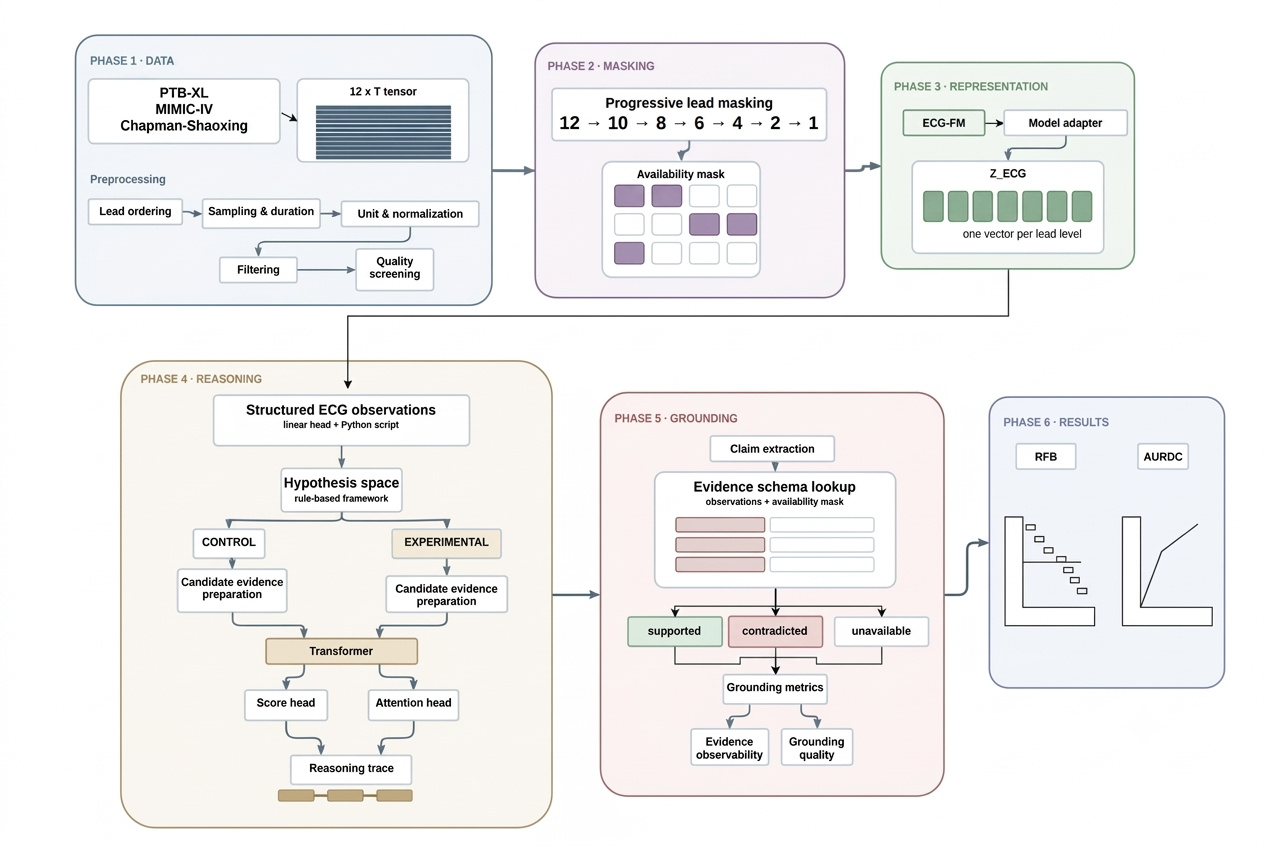
\includegraphics[width=\textwidth]{images/fig3_1_architecture.jpg}
\caption[Architecture of the Proposed System]{Architecture of the Proposed System (the grounding phase, the knowledge-augmented experimental path and the RFB/AURDC analysis are specified but not yet implemented)}
\label{fig:architecture_proposed}
\end{figure}

The implementation status of each component was determined from the source code, configuration files, test suite and run artefacts of the repository, and is summarised in Table~\ref{tab:implementation_status}.

\begin{table}[htbp]
\centering
\scriptsize
\caption{Implementation Status of System Components}
\label{tab:implementation_status}
\renewcommand{\arraystretch}{1.2}
\setlength{\tabcolsep}{3pt}
\setstretch{1.0}
\begin{tabular}{|>{\raggedright\arraybackslash}p{3.7cm}|>{\raggedright\arraybackslash}p{4cm}|>{\raggedright\arraybackslash}p{7cm}|}
\hline
\textbf{Component} & \textbf{Status} & \textbf{Evidence in repository} \\ \hline
Dataset acquisition and label harmonisation (Module 1) & Implemented and tested & \url{runs/module1_v2/} freeze record; \url{labels/label_mapping_rules.json} \\ \hline
Signal preprocessing (Module 1) & Implemented and tested & \url{src/preprocessing/}; \url{tests/test_preprocessing.py} \\ \hline
Patient-disjoint data partitioning (Module 1) & Implemented and tested & \url{runs/module4_v3/split_manifest.csv}; \url{tests/test_gate1_remediation.py} \\ \hline
Lead masking and lead provenance (Module 2) & Implemented and tested & \url{src/degradation/lead_masking.py}; \url{tests/test_lead_masking.py} \\ \hline
Frozen foundation-model representations (Module 3) & Implemented and tested & \url{src/models/ecg_fm_primary.py}; \url{runs/module3_v1/} freeze record \\ \hline
Clinical observation extractor & Implemented, partially evaluated & \url{src/observations/clinical_extractor.py}; known limitations in Section 3.3.7 \\ \hline
Control Reasoning Transformer, training and calibration (Module 4) & Implemented; evaluated for classification only & \url{src/reasoning/}; \url{scripts/16_train_reasoning_transformer.py}; \url{runs/module4_v3/} \\ \hline
Attention-based reasoning traces & Implemented, not validated as explanations & \url{src/reasoning/trace_generator.py}; \url{scripts/17_*}, \url{scripts/18_*} \\ \hline
Grounding gate and evidence states (Module 5) & Defined in protocol, not implemented; evidence schema requires revision before implementation (Section 3.3.9) & \url{reports/module4_evaluation_protocol.md} Section 3; \url{reports/evidence_observability_config.json} \\ \hline
Grounding metrics, RFB, DFB, AURDC (Module 6) & Defined in protocol, not implemented & Protocol Sections 4--7 \\ \hline
Clinical Knowledge Prior and knowledge-augmented path & Proposed future work & Protocol Section 6 (baseline B-4); \url{configs/benchmark_candidates.json} \\ \hline
\end{tabular}
\end{table}

\section{CONTROL REASONING TRANSFORMER ARCHITECTURE}
The Control Reasoning Transformer is the reasoning model of Module 4. It is built from the standard Transformer components of multi-head self-attention and multi-head attention between two sequences \cite{VASWANI2017ATTENTION}, arranged so that each of the eight candidate diagnoses attends separately to the available evidence. The design follows from the research question: a separate query for each candidate diagnosis produces a separate attention distribution over the evidence for that diagnosis, which can later be compared with the evidence the diagnosis actually requires.

For a recording at lead configuration $l$, the model receives three inputs: the foundation-model representation $\mathbf{z} \in \mathbb{R}^{768}$, the structured observations $O_l$ extracted from the available leads, and the binary lead-availability mask $\mathbf{m}_l \in \{0,1\}^{12}$. These are converted into a sequence of $N = 51$ evidence tokens of dimension $d = 256$:

\[
\mathbf{E} = [\,\mathbf{e}_{\text{ECG}};\ \mathbf{e}^{\text{lead}}_{1,\ldots,12};\ \mathbf{e}_{\text{rhythm}};\ \mathbf{e}_{\text{interval}};\ \mathbf{e}^{\text{STE}}_{1,\ldots,12};\ \mathbf{e}^{\text{STD}}_{1,\ldots,12};\ \mathbf{e}^{\text{TWI}}_{1,\ldots,12}\,] \in \mathbb{R}^{51 \times 256}
\]

The first token is a learned projection of $\mathbf{z}$ (a linear layer, layer normalisation, GELU activation and dropout). Each of the twelve lead tokens is the sum of a learned embedding of the lead's position and a learned embedding of its status, active or masked, so the model is told explicitly which leads are absent. The rhythm token is an embedding of the rhythm label produced by the observation extractor, and the interval token is a learned projection of the heart rate, PR interval and QRS duration after standardisation, $(\text{HR}-75)/30$, $(\text{PR}-160)/40$ and $(\text{QRS}-100)/25$, with a missing value set to zero. The remaining 36 tokens represent ST elevation, ST depression and T-wave inversion for each lead: a lead's token is a learned embedding when the finding is present on an active lead, and a zero vector otherwise. All tokens are layer-normalised.

The evidence sequence is encoded by a two-layer Transformer encoder with four attention heads, a feed-forward dimension of 512, GELU activation, pre-layer normalisation and dropout of 0.1. Each encoder layer applies scaled dot-product self-attention,

\[
\operatorname{Attention}(\mathbf{Q},\mathbf{K},\mathbf{V}) = \operatorname{softmax}\!\left(\frac{\mathbf{Q}\mathbf{K}^{\top}}{\sqrt{d_k}}\right)\mathbf{V},
\]

where $\mathbf{Q}$, $\mathbf{K}$ and $\mathbf{V}$ are linear projections of the token sequence and $d_k$ is the dimension of each head \cite{VASWANI2017ATTENTION}. Eight learned query vectors $\mathbf{H} \in \mathbb{R}^{8 \times 256}$, one per candidate diagnosis, then attend to the encoded evidence $\tilde{\mathbf{E}}$ through multi-head cross-attention. The attention weights, averaged over heads, form a matrix $\mathbf{A} \in \mathbb{R}^{8 \times 51}$ in which row $i$ describes how candidate $i$ distributes its attention over the evidence tokens. The attended queries are combined with the original queries through a residual connection, layer normalisation and a feed-forward block, and a score head (a linear layer to 128 units, layer normalisation, GELU, dropout and a linear layer to one output) produces a logit $s_i$ for each candidate. The posterior probability of candidate $i$ is

\[
p_i = \sigma(s_i), \qquad i = 1, \ldots, 8,
\]

where $\sigma$ is the logistic sigmoid. Independent sigmoids are used because the benchmark is multi-label: a recording may show more than one condition, such as atrial fibrillation together with a bundle branch block.

The model has 1,830,657 trainable parameters, about 2\% of the 90.9 million parameters of the frozen foundation model. Its forward method raises an error if Clinical Knowledge Prior tokens are supplied, which enforces the control condition in code. One limitation was identified while preparing this chapter: the rhythm labels written by the observation extractor are spelled differently from the rhythm vocabulary of the context builder. Only ``Sinus rhythm'' matches, so every other rhythm label is mapped to the same out-of-vocabulary embedding. This affects 12,152 of the 25,825 training observations (47.1\%). In the trained model the rhythm token therefore distinguishes only sinus rhythm from all other rhythms; heart rate still reaches the model through the interval token. This defect is reported here rather than corrected, because the trained checkpoints and their evaluation are frozen.

\section{MODULES}
The modules are described below in the order in which data pass through them. For each module, the description states what is implemented, which parameters were used, and which parts remain planned.

\subsection{Dataset Acquisition and Provenance}
Three public 12-lead ECG cohorts are used, each identified by the exact version obtained. PTB-XL is a clinical dataset of 10-second ECGs annotated by cardiologists with SCP-ECG statements \cite{WAGNER2020PTBXL}; the project uses PhysioNet release 1.0.3 \cite{WAGNER2022PTBXLDATA}. Because the original PTB-XL publication describes an earlier release, record counts in this report are taken from version 1.0.3 and from the repository, not from the publication.

The Chapman-Shaoxing database of 12-lead ECGs with expert rhythm labels was created by Chapman University and Shaoxing People's Hospital \cite{ZHENG2020CHAPMAN}. The project did not obtain it from the original distribution. Its files were downloaded from the training set of the PhysioNet/Computing in Cardiology Challenge 2021, release 1.0.3 \cite{REYNA2022ISSUES,CINC2021DATA}, as recorded by the download script (\url{scripts/download_validation_data.py}) and the records manifest (\url{data/external_validation/chapman/records_manifest.csv}). A sample record was checked to be byte-identical to the corresponding Challenge 2021 file. This distribution supplies diagnoses as SNOMED CT codes in the header of each record.

MIMIC-IV-ECG is a collection of diagnostic ECGs matched to the MIMIC-IV clinical database \cite{GOW2023MIMICIVECG}. The project uses release 1.0 and draws a subset of 5,000 recordings, one per patient, sampled with a fixed seed to give approximately equal numbers of records for the eight conditions. The labels of this cohort come from the machine-generated interpretation statements distributed with the dataset, not from cardiologist annotation, which is recorded as a limitation of the cohort.

All three cohorts contribute records to the training, validation and test partitions, so none of them serves as a purely external test cohort. The record counts after quality screening and partitioning are reported in Chapter 4.

\subsection{Benchmark Conditions and Label Harmonisation}
The benchmark consists of eight conditions, listed in Table~\ref{tab:benchmark_conditions} and fixed in the configuration file \url{configs/benchmark_candidates.json}. They span rhythm (atrial fibrillation, sinus bradycardia, sinus tachycardia), conduction (right and left bundle branch block, first-degree atrioventricular block), ischaemic injury (myocardial infarction) and a normal reference class. They were chosen so that the conditions differ in the leads their criteria depend on. Table~\ref{tab:benchmark_conditions} lists the required leads and measurement requirements that the project's evidence schema (\url{reports/evidence_observability_config.json}) assigns to each condition. Rate-based conditions can in principle be assessed from any single lead, whereas bundle branch block and localised infarction depend on particular leads. This contrast is what the progressive lead-removal experiment is designed to expose.

\begin{table}[htbp]
\centering
\scriptsize
\caption{Benchmark Conditions}
\label{tab:benchmark_conditions}
\renewcommand{\arraystretch}{1.2}
\setlength{\tabcolsep}{3pt}
\setstretch{1.0}
\begin{tabular}{|p{1.3cm}|p{2.4cm}|p{3.1cm}|p{6.9cm}|}
\hline
\textbf{Acronym} & \textbf{Condition} & \textbf{Required leads in the project's schema} & \textbf{Measurement requirement in the project's schema} \\ \hline
NORM & Normal ECG & I, II, V1--V6 & Heart rate 60--100 bpm; PR 120--200 ms; QRS below 120 ms; no ST elevation, ST depression or T-wave inversion \\ \hline
AFIB & Atrial fibrillation & II, V1 & RR-interval coefficient of variation above 0.20; no organised P waves \\ \hline
RBBB & Right bundle branch block & V1, V6 & QRS at least 120 ms; $rsR^\prime$ pattern in V1 or wide slurred S wave in V6 \\ \hline
LBBB & Left bundle branch block & I, V1, V6 & QRS at least 120 ms; broad monophasic R and no Q wave in I and V6; broad QS or rS in V1 \\ \hline
SBRAD & Sinus bradycardia & II & Heart rate below 60 bpm with regular sinus P waves \\ \hline
STACH & Sinus tachycardia & II & Heart rate above 100 bpm with regular sinus P waves \\ \hline
1AVB & First-degree atrioventricular block & II & PR interval above 200 ms with 1:1 atrioventricular conduction \\ \hline
MI & Myocardial infarction & Contiguous leads of at least one territory & ST elevation of at least 0.10 mV in two or more contiguous leads, or pathological Q waves \\ \hline
\end{tabular}
\end{table}

The source datasets use different labelling systems: SCP-ECG statements for PTB-XL, SNOMED CT codes for Chapman-Shaoxing and free-text machine statements for MIMIC-IV-ECG. A rule file (\url{runs/module1_v2/labels/label_mapping_rules.json}) maps each to a three-state label for every condition. A label is positive when there is explicit evidence for the condition and negative when the condition can be excluded under a defensible rule. It is unknown when the evidence is ambiguous or absent. For example, an incomplete right bundle branch block makes the RBBB label unknown rather than negative, and atrial flutter makes the AFIB label unknown. Unknown labels are excluded from both the loss and the evaluation through a per-label observation mask, so that the model is neither rewarded nor penalised on cases whose reference label is uncertain. Treating unclear labels as negatives would have mixed label noise into the very errors the project is trying to interpret.

\subsection{Signal Preprocessing}
All recordings are converted to a common representation: a matrix $\mathbf{X} \in \mathbb{R}^{12 \times 1000}$ in millivolts, covering 10 seconds at 100 Hz. The preprocessing pipeline (\url{src/preprocessing/pipeline.py}) applies five steps in a fixed order.

First, raw amplifier counts are converted to millivolts using the gain $g$ and baseline $b$ in each record header, $x_{\text{mV}} = (x_{\text{ADC}} - b)/g$, and values are clipped to $\pm 15$ mV. Second, the channels are reordered into the standard lead order I, II, III, aVR, aVL, aVF, V1--V6. Some project files call this the Cabrera sequence, but the implemented order is the standard one. Third, the signal is filtered at its native 500 Hz sampling rate: a third-order Butterworth high-pass filter at 0.5 Hz removes baseline wander, an IIR notch filter ($Q = 30$) removes power-line interference at 50 Hz for PTB-XL and Chapman-Shaoxing or 60 Hz for MIMIC-IV-ECG, and a fourth-order Butterworth low-pass filter at 45 Hz removes high-frequency noise. Filtering before resampling keeps the 50 and 60 Hz notch frequencies below the Nyquist limit, which would not be the case at 100 Hz. All filters are applied forwards and backwards to avoid phase distortion. Fourth, the signal is resampled from 500 Hz to 100 Hz with polyphase filtering (\texttt{scipy.signal.resample\_poly}, downsampling factor 5), and the central 10-second window is retained. Fifth, quality screening rejects recordings with non-finite values, a flat channel (standard deviation below $10^{-4}$ mV), a flat segment of 1.5 seconds or more, or amplitudes beyond the $\pm 15$ mV limit. Rejected recordings are excluded from all later modules. No amplitude normalisation is applied, so the signals presented to the foundation model are in millivolts.


\subsection{Data Partitioning and Leakage Prevention}
Records are assigned to ten folds by a patient-grouped iterative multi-label stratification procedure with a fixed seed of 42 (\url{runs/module1_v2/scripts/build_stage2_splits.py}). All recordings of a patient are placed in the same fold, and the folds are balanced over the eight labels. Folds 1 to 7 form the training partition, fold 8 the validation partition and folds 9 and 10 the test partition. Patient identifiers are compared across partitions to confirm that no patient appears in more than one. Chapman-Shaoxing does not provide patient identifiers, so each record is treated as its own patient. The Module 1 freeze record lists 13 pairs of identical Chapman-Shaoxing signals stored under different record identifiers; seven test records have exact copies in training or validation data, a small but confirmed leakage described in Section 4.1.2. Because Chapman-Shaoxing has no patient identifiers, patient-level separation is established for PTB-XL and MIMIC-IV-ECG but cannot be established for Chapman-Shaoxing.

The partitions have fixed roles. The training partition is used only for gradient updates. The validation partition is used only for early stopping, model selection and calibration. The test partition is reserved for a single evaluation after all model weights, calibration parameters and evaluation code have been frozen. To make accidental use of test labels less likely, individual test labels are blanked in the Module 4 split manifest, and the data loader refuses to load test data unless the test stage is explicitly requested. The governance of the test evaluation is discussed in Section 3.3.12.

\subsection{Progressive Lead-Availability Configurations and Masking}
Physiological information is removed by applying seven fixed lead-availability configurations, defined in \url{configs/lead_configurations.json} and listed in Table~\ref{tab:lead_configurations}. They retain 12, 10, 8, 6, 4, 2 and 1 leads. The configurations reflect clinical acquisition patterns: the full 12-lead recording, the eight independently measured leads, the six frontal-plane limb leads used by some portable devices, a four-lead monitoring arrangement, a two-lead arrangement of the kind used in telemetry, and a single lead II as recorded in rhythm monitoring. The device associations in the configuration file are motivations rather than reproductions of particular devices.

\begin{table}[htbp]
\centering
\small
\caption{Lead-Availability Configurations}
\label{tab:lead_configurations}
\renewcommand{\arraystretch}{1.2}
\setlength{\tabcolsep}{3pt}
\setstretch{1.0}
\begin{tabular}{|p{1.6cm}|p{3.8cm}|p{4.3cm}|p{4.3cm}|}
\hline
\shortstack{\textbf{Leads}\\\textbf{retained}} & \textbf{Identifier} & \textbf{Active leads} & \textbf{Removed leads} \\ \hline
12 & C12\_FULL & I, II, III, aVR, aVL, aVF, V1--V6 & None \\ \hline
10 & C10\_PREC\_LIMB & I, II, aVR, aVL, V1--V6 & III, aVF \\ \hline
8 & C8\_INDEPENDENT & I, II, V1--V6 & III, aVR, aVL, aVF \\ \hline
6 & C6\_LIMB\_6 & I, II, III, aVR, aVL, aVF & V1--V6 \\ \hline
4 & C4\_EINTHOVEN\_\allowbreak SEPTAL & I, II, III, V1 & aVR, aVL, aVF, V2--V6 \\ \hline
2 & C2\_TELEMETRY & II, V1 & All others \\ \hline
1 & C1\_SINGLE\_LEAD & II & All others \\ \hline
\end{tabular}
\end{table}

For configuration $l$, the binary mask $\mathbf{m}_l \in \{0,1\}^{12}$ marks the active leads, and the degraded recording is

\[
\mathbf{X}_l = \mathbf{X} \odot \left(\mathbf{m}_l \mathbf{1}_{1000}^{\top}\right),
\]

where $\odot$ denotes element-wise multiplication and $\mathbf{1}_{1000}$ is a vector of ones. Removed leads are therefore set exactly to zero, and active leads are left unchanged. Missing leads are not reconstructed. Reconstruction would replace missing measurements with estimates, and deep-learning reconstruction has been shown to regress towards population averages rather than reproduce the individual patient's signal \cite{PRESACAN2025RECON}. A reconstructed lead would therefore blur the distinction between recorded and unrecorded evidence on which the grounding analysis depends. Setting removed leads to zero has its own cost: it changes the input distribution, and degradation measured under removed input can reflect distribution shift as well as information loss \cite{HOOKER2019ROAR}. To reduce this effect, the reasoning model is trained on all seven configurations, as described in Section 3.3.8.

The lead-provenance component records which leads are measured and which are derived. Leads I and II and the six precordial leads are treated as measured. Lead III and the augmented leads are linear combinations of leads I and II \cite{KLIGFIELD2007AHA}:

\[
\text{III} = \text{II} - \text{I}, \quad \text{aVR} = -\tfrac{1}{2}(\text{I} + \text{II}), \quad \text{aVL} = \text{I} - \tfrac{1}{2}\text{II}, \quad \text{aVF} = \text{II} - \tfrac{1}{2}\text{I}.
\]

Each lead in a configuration is labelled as observed and measured, observed and derived with both parents present, derived but lacking a parent, or masked. Two consequences follow for the interpretation of results. The 10-lead and 8-lead configurations remove only derived leads, so they hide information from the model without removing it from the recording. And the configurations are not nested: the 6-lead configuration removes all precordial leads, whereas the 4-lead and 2-lead configurations keep V1. Behaviour across the sequence is therefore not expected to change monotonically.

\subsection{Foundation-Model Representation Extraction}
The foundation model is ECG-FM, an open transformer-based ECG model with about 90.9 million parameters that follows the wav2vec 2.0 architecture \cite{MCKEEN2025ECGFM}. The checkpoint used is the released pretrained model \url{mimic_iv_ecg_physionet_pretrained.pt}. Its architecture was verified directly from the checkpoint: a convolutional feature encoder followed by a 12-layer Transformer encoder with 768-dimensional hidden states, 12 attention heads, a feed-forward dimension of 3,072 and 90,883,072 parameters in total. ECG-FM was pretrained with a hybrid self-supervised method combining wav2vec 2.0 signal masking, the contrastive multi-segment coding objective of CLOCS and random lead masking \cite{MCKEEN2025ECGFM,OH2022LEADAGNOSTIC}. Random lead masking means that the model has already been exposed to recordings with missing leads during pretraining.

All parameters of the foundation model are frozen. Each degraded recording $\mathbf{X}_l$ is passed through the encoder, and the output of the final Transformer layer is averaged over time to give the representation $\mathbf{z}_l \in \mathbb{R}^{768}$. Freezing the model has two purposes. It ensures that differences between the representations of the seven configurations are caused by the removed leads and not by adaptation of the encoder, and it keeps the trainable part of the system small. The similarity between $\mathbf{z}_l$ and the full-lead representation $\mathbf{z}_{12}$ is measured by cosine similarity, $\mathbf{z}_l^{\top}\mathbf{z}_{12} / (\lVert\mathbf{z}_l\rVert\,\lVert\mathbf{z}_{12}\rVert)$, as a measure of representation stability. It is not a measure of diagnostic accuracy.

The conditions under which ECG-FM was pretrained differ from the conditions under which it is used in this project. According to its authors, the model was pretrained on recordings resampled to 500 Hz, cut into 5-second segments and z-score normalised, drawn from MIMIC-IV-ECG and the PhysioNet 2021 challenge collection \cite{MCKEEN2025ECGFM}. The project presents 10-second recordings at 100 Hz in millivolts without normalisation. Pretraining also masked leads at random with a probability of 0.5 per lead, whereas the project removes leads only in the fixed configurations of Table~\ref{tab:lead_configurations}. The representations are therefore obtained outside the model's pretraining conditions, and their quality under these conditions has not been established by the model's authors. In addition, two of the project's cohorts, PTB-XL and Chapman-Shaoxing, belong to the PhysioNet 2021 collection, and MIMIC-IV-ECG was also a pretraining source. Pretraining did not use diagnostic labels, but the encoder may have seen some of the project's test recordings; record-level overlap has not been verified. Both points are treated as limitations in Chapters 4 and 5.


\subsection{Clinical Observation Extraction}
The observation extractor (\url{src/observations/clinical_extractor.py}) computes physiological measurements using only the leads that are active in the current configuration. Its outputs serve two purposes: they are tokens for the reasoning model, and they are intended as the measured evidence for the grounding gate.

Heart rate is computed with a simplified detector in the style of the Pan--Tompkins algorithm \cite{PAN1985QRS}. The signal is band-pass filtered between 5 and 15 Hz with a second-order Butterworth filter, differentiated, squared and integrated over a 100 ms moving window. R peaks are then detected as peaks above a fixed threshold of the mean plus 1.5 standard deviations of the integrated signal, at least 250 ms apart, and refined to the local maximum of the raw signal within 50 ms. Unlike the original, it uses a fixed threshold and runs at 100 Hz, so the detection performance reported for the original algorithm does not apply to it. The rhythm lead is the first available of II, V1, I and V5. Because lead II is retained in all seven configurations (Table~\ref{tab:lead_configurations}), heart rate, rhythm, PR interval and QRS duration are always computed from lead II and are identical across configurations; only the per-lead ST and T-wave findings change with lead removal. The rhythm is classed as irregular, a proxy for atrial fibrillation, when the coefficient of variation of the RR intervals exceeds 0.20; otherwise it is sinus bradycardia below 60 beats per minute, sinus tachycardia above 100 beats per minute, and sinus rhythm in between.

Interval and morphology measurements are taken around each detected R peak. The QRS duration is estimated from the minima within 60 ms either side of the peak. Because this window spans at most 110 ms at 100 Hz, the extractor cannot report a QRS duration of 120 ms or more, so the bundle branch block criterion of Table~\ref{tab:benchmark_conditions} can never be satisfied by the current extractor. The PR interval is estimated as the time from the largest deflection between 250 and 60 ms before the R peak to the R peak itself; this is a heuristic and not the clinical PR interval measured from the onset of the P wave to the onset of the QRS complex. ST deviation is measured 60 ms after the R peak relative to a baseline 120 ms before it, and the median over beats is compared with thresholds of +0.10 mV for elevation and $-0.05$ mV for depression. T-wave inversion is recorded when the median amplitude 200 ms after the R peak, relative to the same baseline, is below $-0.10$ mV. Masked leads are excluded from every measurement, and findings are reported only for active leads, so the absence of a finding on a masked lead is never recorded as a normal result. Its unit tests do not check measurement accuracy; its agreement with machine measurements on 250 MIMIC-IV-ECG recordings, obtained with the frozen extractor code, is examined in Section 4.4.8.

\subsection{Training, Calibration and Reasoning Traces}
The Control Reasoning Transformer is trained on the foundation-model representations and observations of the training partition, with every recording presented in all seven configurations in each epoch. A single model therefore learns to operate across all levels of lead availability, instead of one model being trained for each configuration. The loss is a binary cross-entropy restricted to labels that are known:

\[
\mathcal{L} = \frac{1}{\sum_{n,i} o_{n,i}} \sum_{n,i} o_{n,i} \left[-y_{n,i}\log p_{n,i} - (1-y_{n,i})\log(1-p_{n,i})\right],
\]

where $y_{n,i} \in \{0,1\}$ is the label of recording $n$ for condition $i$, $p_{n,i}$ is the predicted probability, and $o_{n,i} \in \{0,1\}$ is the label observation mask of Section 3.3.2. Training uses the AdamW optimiser with a learning rate of $10^{-4}$, weight decay of $10^{-4}$, a batch size of 64, and a cosine learning-rate schedule over at most 15 epochs without warm-up. These settings are confirmed by the saved run; the training configuration file lists different values that the script does not apply (Section 4.2). Training stops early when the validation loss does not improve by at least $5 \times 10^{-4}$ for five epochs, and the checkpoint with the lowest validation loss is retained. The model is trained with three random seeds (42, 1337 and 2024). Seed 42 is the primary model and the other two are used to estimate variability.

The predicted probabilities are calibrated by temperature scaling. Guo et al. introduced temperature scaling as a single scalar temperature that divides the logits of a softmax classifier, fitted by minimising the negative log-likelihood on validation data \cite{GUO2017CALIBRATION}. Because the present model produces eight independent sigmoid outputs, the project adapts this method by fitting a separate temperature $T_i$ for each condition. The calibrated probability is

\[
\hat{p}_i = \sigma\!\left(s_i / T_i\right),
\]

with $T_i \in [0.1, 10]$ chosen by bounded scalar minimisation of the negative log-likelihood on the validation partition. This per-condition, sigmoid-based variant is the project's adaptation and not a reproduction of the original method. Calibration is measured by the expected calibration error over 10 equal-width probability bins \cite{GUO2017CALIBRATION},

\[
\text{ECE} = \sum_{b=1}^{10} \frac{|B_b|}{n}\,\bigl|\operatorname{acc}(B_b) - \operatorname{conf}(B_b)\bigr|,
\]

where $B_b$ is the set of predictions in bin $b$, $\operatorname{acc}(B_b)$ is the fraction of positive labels in the bin and $\operatorname{conf}(B_b)$ is the mean predicted probability in the bin.

For each recording and configuration, a trace generator (\url{src/reasoning/trace_generator.py}) produces a structured reasoning trace. The trace records the calibrated probabilities, the single highest-probability hypothesis, the evidence tokens to which that hypothesis attended with a weight of at least 0.02 (up to five tokens for validation traces and four for test traces), the leads associated with each token and whether those leads were active, and a heart-rate contradiction check for sinus bradycardia and sinus tachycardia. Attention weights show where the model routed information, not why it reached its decision, and they cannot be assumed to be faithful explanations \cite{JAIN2019ATTENTION}. For this reason the traces are treated as candidate claims to be checked by the grounding gate, not as verified explanations. The current traces are not yet usable as claims: each traces only the single highest-probability hypothesis, even when it falls below the decision threshold (14.1\% of the 25,816 validation traces) or when the recording has several positive predictions (12.1\%), and most selected tokens encode only a lead's position and status rather than a finding. The procedure for converting traces into verifiable clinical claims has not yet been defined, and the trace-quality labels written by the validation-trace script come from ad hoc rules, not from the grounding gate.

\subsection{Evidence States and the Grounding Gate}
The grounding gate is the component that will decide, for each clinical claim in a reasoning trace, whether the claim is supported by the available evidence. It is specified in the project's internal evaluation protocol and in an evidence schema (\url{reports/evidence_observability_config.json}) but has not yet been implemented. For each condition, the schema lists the leads required to assess a claim, the measurement rule that the claim must satisfy, and the condition under which the claim is unavailable. The schema is grounded in the AHA/ACCF/HRS recommendations for conduction disturbances and for acute ischaemia and infarction \cite{SURAWICZ2009AHA,WAGNER2009AHA}. Its specific thresholds and lead requirements, summarised in Table~\ref{tab:benchmark_conditions}, are the project's operational choices. Several of these requirements depend on waveform morphology, such as the $rsR^\prime$ pattern of right bundle branch block, which the current observation extractor does not measure, so the extractor will have to be extended before the gate can be implemented for those conditions. A review of the schema for this chapter found further issues that must be resolved before implementation: the required leads of left bundle branch block, sinus bradycardia, sinus tachycardia, first-degree atrioventricular block and myocardial infarction disagree with their unavailability rules; some verification and contradiction rules leave cases undecided (a QRS duration between 100 and 120 ms satisfies neither rule for bundle branch block); the atrial fibrillation rule is satisfied whenever V1 is active; P-wave, QRS-morphology, Q-wave and signal-quality measurements are not produced by the extractor; the normal-ECG QRS requirement is always met because of the QRS limit; and the protocol does not say how to treat missing measurements, claims with several findings or alternative criteria, such as ST elevation or Q waves for infarction. These are design decisions for the researcher; none of them is resolved in this report.

Let $\mathcal{L}_{\text{req}}(f_k)$ be the set of leads required to assess finding $f_k$ in claim $C_k$, and let $\theta(f_k)$ be its measurement rule. The gate assigns each claim exactly one of three states, as shown in Algorithm~\ref{alg:grounding_gate}. A claim is UNAVAILABLE when any required lead is masked, SUPPORTED when all required leads are active and the measurements satisfy the rule, and CONTRADICTED when all required leads are active but the measurements do not satisfy it. For myocardial infarction, the schema accepts ST elevation in two or more contiguous leads or pathological Q waves, and it requires at least two active contiguous leads within one anatomical territory: II, III and aVF (inferior); V1 and V2 (septal); V3 and V4 (anterior); or I, aVL, V5 and V6 (lateral). The rule is not relaxed when fewer leads are available, so every infarction claim in the 2-lead and 1-lead configurations is UNAVAILABLE.

\begin{algorithm}[htbp]
\caption{Grounding Gate (specified, not yet implemented)}
\label{alg:grounding_gate}
\footnotesize
\begin{verbatim}
Input:  reasoning trace with claims C_1 ... C_K;
        lead mask m_l; measured observations O_l
Output: verdict V(C_k) in {SUPPORTED, CONTRADICTED,
        UNAVAILABLE} for each claim

for each claim C_k asserting finding f_k:
    if any lead j in L_req(f_k) has m_l[j] = 0:
        V(C_k) <- UNAVAILABLE
        # required evidence was not recorded
    else if O_l satisfies theta(f_k):
        V(C_k) <- SUPPORTED
        # evidence present and consistent
    else:
        V(C_k) <- CONTRADICTED
        # evidence present and inconsistent
return V(C_1) ... V(C_K)
\end{verbatim}
\normalsize
\end{algorithm}

The three states are mutually exclusive, so the number of claims at configuration $l$ satisfies $N_{\text{total},l} = N_{\text{sup},l} + N_{\text{con},l} + N_{\text{una},l}$. The most important property of the gate is that a claim is never marked CONTRADICTED merely because its leads are absent. Missing evidence is kept separate from evidence that conflicts with the claim. A comparable distinction is made in text fact-verification, where FEVER labels claims as Supported, Refuted or NotEnoughInfo with respect to retrieved evidence \cite{THORNE2018FEVER}. The UNAVAILABLE state is the project's own adaptation of this distinction: it is determined by lead availability and is not equivalent to FEVER's NotEnoughInfo category.

\subsection{Clinical Knowledge Prior}
The Clinical Knowledge Prior (CKP) is a proposed extension of the reasoning stage and is planned future work. Its purpose is to supply the reasoning model with structured clinical knowledge about which findings and which leads each diagnosis requires, so that it can be tested whether such knowledge changes the configuration at which reasoning stops being grounded. The knowledge would be organised using SNOMED CT, the clinical terminology that the benchmark already uses to identify its eight conditions and whose encoded concepts can be combined with patient data in decision-support systems \cite{SNOMED2026CDSGUIDE}. Recent work has combined clinical knowledge with variable-lead ECG representation learning \cite{LIU2025ARBITRARY}. That work uses knowledge to improve representations, whereas the proposed CKP would serve as a reference against which claims are checked.

The knowledge-augmented path must score exactly the same eight candidate diagnoses as the control path, without filtering or re-ranking them, and it appears in the protocol only as a planned comparison (B-4). The CKP has not been implemented, and no such comparison is reported here.

\subsection{Evaluation Metrics and the Reasoning Failure Boundary}
Evaluation is carried out separately for each of the seven configurations, using the calibrated probabilities. Diagnostic performance is measured, for each condition, by the area under the receiver operating characteristic curve (AUROC) and by the F1 score at a decision threshold of 0.5, computed only over records whose label for that condition is known. The macro averages over the eight conditions summarise performance for a configuration. Calibration is measured by the Brier score, the negative log-likelihood and the expected calibration error of Section 3.3.8. Confidence intervals for macro-AUROC and macro-F1 are obtained from 200 bootstrap resamples of records, using the 2.5th and 97.5th percentiles. These resamples are drawn at the record level and do not group the recordings of a patient. This differs from the protocol, which specifies 1,000 patient-clustered resamples for the grounding metrics.

The grounding metrics are defined in the protocol and will be computed once the gate is implemented. For configuration $l$, let $N_{\text{req},l}$ be the number of evidence criteria required by the claims, and $N_{\text{obs},l}$ the number of those criteria whose leads are all active. Then

\[
\text{EO}_l = \frac{N_{\text{obs},l}}{N_{\text{req},l}}, \qquad \text{GQ}_l = \frac{N_{\text{sup},l}}{N_{\text{sup},l} + N_{\text{con},l}}, \qquad \text{TGR}_l = \text{GQ}_l \times \text{EO}_l,
\]

\[
\text{UR}_l = \frac{N_{\text{una},l}}{N_{\text{total},l}}, \qquad \text{GSR}_l = \frac{N_{\text{sup},l}}{N_{\text{total},l}}.
\]

Evidence observability (EO) describes how much of the required evidence the configuration exposes. Grounding quality (GQ) is the proportion of supported claims among the claims that can be assessed. The true grounding ratio (TGR) combines the two. The unavailable ratio (UR) and the grounded support ratio (GSR) describe the full set of claims. GQ is reported as not estimable when no claim can be assessed, rather than being set to zero or one. Counts are summed over all test records before the ratios are formed; per-record averages are reported as a secondary analysis.

The Reasoning Failure Boundary (RFB) is defined over the ordered sequence of configurations $\mathcal{S} = \langle 12, 10, 8, 6, 4, 2, 1 \rangle$ as the first configuration $c_k$ at which grounding quality falls below a threshold $\tau$:

\[
c_{\text{RFB}}(\tau) = \text{first } c_k \in \mathcal{S} \text{ such that } \text{GQ}(c_k) < \tau.
\]

The primary threshold is $\tau = 0.60$, with 0.50 and 0.70 as sensitivity values. These are analysis parameters chosen by the project, not clinical standards. The boundary is reported as a transition from the last acceptable configuration to the first failing one, and the full vector of GQ values over the seven configurations is always reported. Because the configurations are not nested, grounding quality may fall below the threshold at one configuration and recover at a later one, for example when the 4-lead configuration regains lead V1 after the 6-lead configuration has removed all precordial leads. In that case the initial failure is reported, the recovery is flagged, and the sustained boundary after which GQ never recovers is reported as well; the protocol also defines robust, failed-at-baseline and indeterminate outcomes. Because GQ excludes UNAVAILABLE claims, at low lead counts it may rest on the few claims that remain assessable, such as rate-based claims on lead II. A configuration in which most claims are unavailable can therefore still pass the GQ threshold, and the boundary has to be read together with UR and TGR.

The Diagnostic Failure Boundary (DFB) is defined analogously from the retained performance ratio $\text{RPR}(c_k) = \text{macro-F1}(c_k)/\text{macro-F1}(c_{12})$, as the first configuration at which RPR falls below 0.80. The decoupling between the two boundaries is expressed as an ordinal step gap, $\Delta_{\text{steps}} = k_{\text{DFB}} - k_{\text{RFB}}$, where $k$ is the position of a configuration in $\mathcal{S}$, and as a lead-count gap, $\Delta_{\text{leads}} = l_{\text{RFB}} - l_{\text{DFB}}$. A positive gap means that diagnostic performance survives further down the sequence than grounded reasoning. Whether such a gap exists is a hypothesis to be tested. Finally, the area under the reasoning degradation curve summarises grounding quality across the sequence by trapezoidal integration over the lead counts $l_k$, normalised to the unit interval:

\[
\text{AURDC} = \frac{1}{11}\sum_{k=1}^{6} \frac{\text{GQ}(c_k) + \text{GQ}(c_{k+1})}{2}\,(l_k - l_{k+1}).
\]

The protocol does not define how to handle a non-estimable GQ inside the sequence, and the DFB, RPR, their bootstrap intervals and any paired comparison of configurations are not yet implemented.

The protocol defines four comparison models. The linear probe on the frozen foundation-model representation (B-1) has been evaluated for classification only; its evaluation script is not in the repository and its per-record predictions were not saved, so comparisons with it are descriptive. The result of the rule engine that applies the evidence criteria directly (B-2) has been withdrawn, because the QRS limitation of Section 3.3.7 made its bundle branch block rules unsatisfiable. The Control Reasoning Transformer (B-3) is implemented and evaluated for classification, but its grounding has not yet been evaluated. Knowledge-augmented reasoning with the Clinical Knowledge Prior (B-4) is planned.


\subsection{Reproducibility and Evaluation Governance}
The design, metrics and boundary rules of Sections 3.3.9 to 3.3.11 are fixed in an internal evaluation protocol, version 2.0, dated 14 October 2026, which labels itself ``PRE-REGISTERED''. A SHA-256 hash of the protocol was recorded in the Module 4 freeze record (\url{runs/module4_v3/MODULE4_FROZEN.json}) on 15 October 2026 at 06:54 UTC, and it matches the current file. The same record holds hashes of the training configuration, the lead configurations, the benchmark definition, the evidence schema, the main source files and the checkpoints of all three seeds. No external registration of the protocol has been identified, so the protocol is an internal, hash-verified document rather than an externally registered one. Of the files listed in the freeze record, one source file (\url{src/reasoning/multi_cohort_loader.py}) has changed since the record was made. Its last modification, at 16:08 UTC on 15 October 2026, falls after the freeze and before the test evaluation finished. The test evaluation was therefore run with a data loader that differs from the frozen version, and the test-trace script is not listed in the freeze record at all.

The protocol requires the test partition to be evaluated once, after explicit authorisation by the investigator. The project's provenance statement (\url{runs/module4_v3/reports/evaluation_provenance_statement.md}) records that this condition was not met, so the test evaluation, completed on 15 October 2026 at 16:29 UTC, is classified as authorisation-unverified; Section 4.3.2 gives the details. The test results in Chapter 4 are therefore descriptive measurements, not a confirmatory pre-specified evaluation, and any authorised re-evaluation must be a new, separately versioned run.
 % DESIGN
\chapter{EXPERIMENTAL RESULTS AND PERFORMANCE ANALYSIS}
\label{chap:ch4}





\section{DATASET DESCRIPTION}\label{sec:ch4_1}

\subsection{Source Datasets and Versions}\label{sec:ch4_1_1}

The project pools three public 12-lead ECG cohorts, each identified by the exact release obtained (Section 3.3.1). Table~\ref{tab:ch4_1} gives, for each cohort, the release, the source of its diagnostic labels and the number of recordings at each stage of preparation. The counts are those written by the preprocessing stage (\url{data/processed_100hz/preprocessing_summary.json} and the per-cohort summaries) and confirmed by a recount of the Module 4 split manifest (\url{runs/module4_v3/split_manifest.csv}).

{
\setlength{\tabcolsep}{2pt}
\renewcommand{\arraystretch}{1.12}
\begin{table}[htbp]
\centering
\scriptsize
\setstretch{1.0}
\caption{Source Datasets Used in the Project}\label{tab:ch4_1}
\begin{tabular}{|p{0.12\textwidth}|p{0.20\textwidth}|p{0.20\textwidth}|p{0.13\textwidth}|p{0.16\textwidth}|p{0.12\textwidth}|}
\hline
\textbf{Cohort} & \textbf{Release used} & \textbf{Source of diagnostic labels} & \textbf{Recordings processed} & \textbf{Rejected by quality screening} & \textbf{Eligible recordings} \\ \hline
PTB-XL & PhysioNet release 1.0.3 \cite{WAGNER2022PTBXLDATA}; dataset described in \cite{WAGNER2020PTBXL} & SCP-ECG statements assigned by cardiologists \cite{WAGNER2020PTBXL} & 21,799 & 2 & 21,797 \\ \hline
Chapman-Shaoxing & Training set of the PhysioNet/Computing in Cardiology Challenge 2021, release 1.0.3, \url{chapman_shaoxing} subset \cite{CINC2021DATA}; original database \cite{ZHENG2020CHAPMAN} & SNOMED CT codes in the record headers & 10,158 & 16 & 10,142 \\ \hline
MIMIC-IV-ECG & Release 1.0 \cite{GOW2023MIMICIVECG}; subset of 5,000 recordings, one per patient, sampled with seed 42 & Machine-generated interpretation statements distributed with the dataset & 5,000 & 51 & 4,949 \\ \hline
\textbf{Total} &  &  & \textbf{36,957} & \textbf{69} & \textbf{36,888} \\ \hline
\end{tabular}
\end{table}
}

The counts in Table~\ref{tab:ch4_1} describe the project's working subset, which differs from the full releases in two ways. For Chapman-Shaoxing, the records manifest (\url{data/external_validation/chapman/records_manifest.csv}) lists 10,247 recordings, of which 89 had missing files, leaving the 10,158 processed recordings. For MIMIC-IV-ECG, the project's sampling audit (\url{reports/dataset_sampling_audit.json}) records a pool of 800,035 recordings from 161,352 patients, from which the 5,000-recording subset was drawn. PTB-XL release 1.0.3 contains 21,799 recordings, all of which were processed.

The three cohorts were labelled in different ways, and this affects how their results can be compared. PTB-XL labels come from cardiologists. Chapman-Shaoxing labels are diagnosis codes supplied with the Challenge 2021 distribution. MIMIC-IV-ECG labels are derived from the statements of an automated interpretation program, so they show what that program reported, not a clinician's diagnosis. Differences in labelling practice and population between ECG databases are a known source of difficulty for multi-database classification \cite{REYNA2022ISSUES}. The per-cohort results of Section~\ref{sec:ch4_4_5} have to be read with this in mind.

\subsection{Data Partitions}\label{sec:ch4_1_2}

The recordings were divided into training, validation and test partitions by the patient-grouped, label-stratified procedure of Section 3.3.4. Table~\ref{tab:ch4_2} gives the number of recordings and patients in each partition, recounted from the Module 4 split manifest.

\begin{table}[htbp]
\centering
\small
\renewcommand{\arraystretch}{1.12}
\setstretch{1.0}
\setlength{\tabcolsep}{2pt}
\caption{Recordings and Patients in Each Partition}\label{tab:ch4_2}
\begin{tabular}{|p{0.25\textwidth}|p{0.18\textwidth}|p{0.18\textwidth}|p{0.18\textwidth}|p{0.14\textwidth}|}
\hline
\textbf{Cohort} & \textbf{Training (folds 1–7)} & \textbf{Validation (fold 8)} & \textbf{Test (folds 9–10)} & \textbf{Total} \\ \hline
PTB-XL recordings & 15,260 & 2,179 & 4,358 & 21,797 \\ \hline
PTB-XL patients & 13,253 & 1,885 & 3,729 & 18,867 \\ \hline
Chapman-Shaoxing recordings (each treated as one patient) & 7,100 & 1,014 & 2,028 & 10,142 \\ \hline
MIMIC-IV-ECG recordings (one per patient) & 3,465 & 495 & 989 & 4,949 \\ \hline
\textbf{All recordings} & \textbf{25,825} & \textbf{3,688} & \textbf{7,375} & \textbf{36,888} \\ \hline
\textbf{All patients} & \textbf{23,818} & \textbf{3,394} & \textbf{6,746} & \textbf{33,958} \\ \hline
Recording–configuration examples (× 7 configurations) & 180,775 per epoch & 25,816 & 51,625 & 258,216 \\ \hline
\end{tabular}
\end{table}

Each recording is presented in all seven lead configurations, so the 51,625 test examples are seven views of 7,375 recordings from 6,746 patients. They are not 51,625 independent patients, and all test sample sizes in this chapter should be read in that light.

No patient identifier appears in more than one partition, but this check only has force where identifiers exist. PTB-XL and MIMIC-IV-ECG provide patient identifiers. Chapman-Shaoxing does not, so each of its recordings is treated as a separate patient and patient-level separation cannot be established for this cohort. The Module 1 freeze record lists 13 pairs of identical Chapman-Shaoxing signals stored under different record identifiers. The labels of each pair agree. Nine of the pairs cross partitions: six link the training and test partitions, two the training and validation partitions, and one the validation and test partitions. Seven test recordings therefore have exact copies in data used for training or model selection. This is about 0.1\% of the 7,375 test recordings, too few to change the reported metrics in any material way, but it is a genuine leakage and is disclosed as such.

\subsection{Label Distribution}\label{sec:ch4_1_3}

Labels have three states: positive, negative and unknown (Section 3.3.2). Unknown labels are excluded from training and evaluation, so each condition is evaluated on its own subset of recordings. Table~\ref{tab:ch4_3} gives the number of positive labels and the number of known labels for each condition in each partition. The test counts come from the confusion matrices in the saved test summary (\url{runs/module4_v3/metrics/test_evaluation_summary.json}), because test labels are blanked in the split manifest as a quarantine measure.

\begin{table}[htbp]
\centering
\small
\setlength{\tabcolsep}{2pt}
\renewcommand{\arraystretch}{1.12}
\setstretch{1.0}
\caption{Positive Labels / Known Labels (Prevalence) in Each Partition}\label{tab:ch4_3}
\begin{tabular}{|p{0.15\textwidth}|p{0.26\textwidth}|p{0.26\textwidth}|p{0.26\textwidth}|}
\hline
\textbf{Condition} & \textbf{Training} & \textbf{Validation} & \textbf{Test} \\ \hline
NORM & 7,889 / 25,730 (30.7\%) & 1,128 / 3,675 (30.7\%) & 2,225 / 7,347 (30.3\%) \\ \hline
AFIB & 2,716 / 25,212 (10.8\%) & 389 / 3,610 (10.8\%) & 788 / 7,188 (11.0\%) \\ \hline
RBBB & 1,177 / 24,094 (4.9\%) & 167 / 3,416 (4.9\%) & 336 / 6,870 (4.9\%) \\ \hline
LBBB & 963 / 24,797 (3.9\%) & 135 / 3,536 (3.8\%) & 274 / 7,089 (3.9\%) \\ \hline
SBRAD & 3,701 / 21,982 (16.8\%) & 528 / 3,132 (16.9\%) & 1,056 / 6,240 (16.9\%) \\ \hline
STACH & 2,156 / 21,980 (9.8\%) & 304 / 3,133 (9.7\%) & 622 / 6,237 (10.0\%) \\ \hline
1AVB & 995 / 22,414 (4.4\%) & 141 / 3,201 (4.4\%) & 286 / 6,368 (4.5\%) \\ \hline
MI & 4,097 / 22,712 (18.0\%) & 584 / 3,255 (17.9\%) & 1,196 / 6,517 (18.4\%) \\ \hline
\end{tabular}
\end{table}

The stratified split keeps the prevalence of every condition almost identical across the three partitions. The conditions are strongly imbalanced, from about 4\% for left bundle branch block and first-degree atrioventricular block to about 30\% for the normal ECG. The test partition still contains at least 274 positive recordings for every condition, so no per-condition test estimate rests on a very small number of positives. The number of known labels differs by condition, from 6,237 to 7,347 test recordings, and per-condition results are therefore computed over different denominators.

\section{ECOSYSTEM (HARDWARE \& SOFTWARE SPECIFICATIONS)}\label{sec:ch4_2}

The repository has no environment file, package list or saved training log. The specifications in Table~\ref{tab:ch4_4} are therefore limited to what can be established from scripts, run reports and checkpoints. Where a specification is not recorded, the table says so rather than inferring it.

\clearpage
{\small
\setlength{\tabcolsep}{2pt}
\renewcommand{\arraystretch}{1.1}
\setstretch{1.0}
\renewcommand{\UrlFont}{\footnotesize\ttfamily}
\setlength{\LTcapwidth}{\textwidth}
\begin{longtable}{|>{\raggedright\arraybackslash}p{0.18\textwidth}|>{\raggedright\arraybackslash}p{0.47\textwidth}|>{\raggedright\arraybackslash}p{0.28\textwidth}|}
\caption{Hardware, Software and Training Specifications}\label{tab:ch4_4}\\
\hline
\textbf{Item} & \textbf{Specification} & \textbf{Evidence} \\ \hline
\endfirsthead
\multicolumn{3}{c}{\tablename~\thetable{} - continued from previous page} \\ \hline

\endhead
\hline
\multicolumn{3}{r}{} \\
\endfoot
\hline
\endlastfoot
Processor and accelerator used for training & Not recorded in the available experiment artefacts. The Stage 6 report states that 16-thread CPU execution was enabled for Module 4; the training script enables this setting only when it runs on the CPU & \url{runs/module4_v3/reports/stage6_validation_and_audit_report.md}; \url{scripts/16_train_reasoning_transformer.py} \\ \hline
Foundation-model feature extraction & CPU; the extraction script fixes the device to the CPU, and the logs record batch size 32 with 8 threads per worker & \url{runs/module3_v1/scripts/extract_foundation_representations.py}; \url{runs/module3_v1/logs/} \\ \hline
Inference for validation traces & CPU, 16-thread worker pool & \url{runs/module4_v3/reports/validation_trace_generation_report.md} \\ \hline
Memory (RAM, accelerator memory) & Not recorded in the available experiment artefacts & — \\ \hline
Operating system & Windows (test session platform \url{win32}) & Stage 6 report, test-suite output \\ \hline
Python & 3.11.4; pytest 9.1.1 & Stage 6 report, test-suite output \\ \hline
Library versions used for the runs & Not recorded in the available experiment artefacts. The Python 3.11.4 installation on the project machine had PyTorch 2.14.0 (CPU build) when this report was written, but this is not evidence of the version used for the runs & Checked on 19 October 2026 \\ \hline
Foundation model & ECG-FM \cite{MCKEEN2025ECGFM}, \url{wav2vec2_cmsc}, 12 encoder layers, width 768; 90,883,072 parameters, all frozen; checkpoint \url{checkpoints/ecg_fm/mimic_iv_ecg_physionet_pretrained.pt} (SHA-256 beginning \url{4d0142bc}) & \url{configs/control_path_training_config.json}; Module 4 freeze record \\ \hline
Control Reasoning Transformer & 1,830,657 trainable parameters & \url{configs/control_path_training_config.json}; checkpoints \\ \hline
Loss & Binary cross-entropy over known labels (Section 3.3.8) & \url{scripts/16_train_reasoning_transformer.py} \\ \hline
Optimiser & AdamW; learning rate $10^{-4}$; weight decay $10^{-4}$; betas (0.9, 0.999) & Checkpoint optimiser state \\ \hline
Batch size & 64 & Checkpoint step count; script default; Stage 6 report \\ \hline
Learning-rate schedule & Cosine annealing over 15 epochs to $10^{-6}$, no warm-up & Learning-rate history in \url{control_training_history_seed*.json} \\

\end{longtable}
}

The training settings in Table~\ref{tab:ch4_4} are those that the run actually used. The training configuration file specifies a batch size of 32, at most 20 epochs and two warm-up epochs, but the training script uses its own defaults of 64, 15 and none. The saved run confirms this: the seed-42 optimiser state shows 2,825 steps per epoch, which is 180,775 examples in batches of 64, and the recorded learning rates follow a 15-epoch cosine schedule from $10^{-4}$ to $10^{-6}$ without warm-up.


\section{EXPERIMENTS CONDUCTED}\label{sec:ch4_3}

\subsection{Overview of the Experiments}\label{sec:ch4_3_1}

Table~\ref{tab:ch4_5} lists the experiments that were carried out, with the artefact that holds each result, its completion status and its main caveat. An experiment is listed as completed only when its saved output was inspected; the existence of a script was not taken as evidence that it ran.

\clearpage
{\small
\setlength{\tabcolsep}{2pt}
\renewcommand{\arraystretch}{1.0}
\setstretch{1.0}
\renewcommand{\UrlFont}{\footnotesize\ttfamily}
\setlength{\LTcapwidth}{\textwidth}
\begin{longtable}{|>{\raggedright\arraybackslash}p{0.08\textwidth}|>{\raggedright\arraybackslash}p{0.20\textwidth}|>{\raggedright\arraybackslash}p{0.24\textwidth}|>{\raggedright\arraybackslash}p{0.18\textwidth}|>{\raggedright\arraybackslash}p{0.21\textwidth}|}
\caption{Experiments Conducted}\label{tab:ch4_5}\\
\hline
\textbf{No.} & \textbf{Experiment} & \textbf{Evidence artefact} & \textbf{Status} & \textbf{Key caveat} \\ \hline
\endfirsthead
\multicolumn{5}{c}{\tablename~\thetable{} - continued from previous page} \\ \hline
\textbf{No.} & \textbf{Experiment} & \textbf{Evidence artefact} & \textbf{Status} & \textbf{Key caveat} \\ \hline
\endhead
\hline
\multicolumn{5}{r}{Continued on next page} \\
\endfoot
\hline
\endlastfoot
E1 & Dataset preparation and quality screening & \url{data/processed_100hz/*/preprocessing_summary.json}; split manifest & Completed: 36,888 of 36,957 recordings retained & Chapman-Shaoxing has no patient identifiers; 13 duplicate pairs \\ \hline
E2 & Progressive lead masking and representation extraction & \url{runs/module3_v1/} (freeze record, logs, drift reports) & Completed: 258,216 representations, no failures recorded & Input conditions differ from ECG-FM pretraining (Section 3.3.6) \\ \hline
E3 & Clinical observation extraction & \url{runs/module4_v3/observations/} & Completed for all partitions and configurations & QRS measurement ceiling; rhythm-label mismatch (Section~\ref{sec:ch4_4_8}) \\ \hline
E4 & Observation-extractor validation study & \url{reports/clinical_observation_validation.json} & Completed: 250 MIMIC-IV-ECG recordings & Reference values are machine measurements, not clinician readings \\ \hline
E5 & Control Reasoning Transformer training & \url{runs/module4_v3/metrics/control_training_history_seed*.json}; checkpoints & Completed for seeds 42, 1337 and 2024 & Settings differ from the configuration file (Section~\ref{sec:ch4_2}) \\ \hline
E6 & Calibration & Training histories & Completed on the validation partition & Fitted and measured on the same validation data \\ \hline
E7 & Validation evaluation by configuration & Training histories & Completed for all three seeds & Uncalibrated probabilities \\ \hline
E8 & Test evaluation of the Control Reasoning Transformer (B-3) & \url{runs/module4_v3/metrics/test_evaluation_summary.json}; \url{test_predictions_seed42.csv} & Completed for seed 42 only & Authorisation-unverified (Section~\ref{sec:ch4_3_2}) \\ \hline
E9 & Comparison models on the test partition & \url{runs/module4_v3/metrics/comprehensive_baseline_comparison.json} & Completed after E8 & Script outside the repository; no per-recording predictions; B-2 defective \\ \hline
E10 & Representation drift & \url{runs/module3_v1/reports/module3_cosine_similarity_summary.csv} & Completed for all partitions & Measures geometry, not diagnostic accuracy \\ 
\end{longtable}
}

The following parts of the research programme were not carried out in the first half and have no results in this chapter:

\begin{itemize}
\item \textbf{Grounding gate and evidence states (Module 5).} Specified in the internal protocol and evidence schema, not implemented. Section 3.3.9 lists the schema revisions required before implementation.
\item \textbf{Grounding metrics (EO, GQ, TGR, UR, GSR) and the Reasoning Failure Boundary (Module 6).} Not computed, because they need the gate's evidence states.
\item \textbf{Diagnostic Failure Boundary and AURDC.} Not implemented in the evaluation scripts. Section~\ref{sec:ch4_4_3} explains why no DFB is read off the classification results.
\item \textbf{Clinical Knowledge Prior and the knowledge-augmented comparison (B-4).} Planned future work.
\item \textbf{Test evaluation of seeds 1337 and 2024, patient-clustered and paired confidence intervals, and ablations of the observation and lead-availability tokens.} Not run.
\end{itemize}

\subsection{Evaluation Provenance}\label{sec:ch4_3_2}

The protocol requires the test partition to be evaluated once, after an explicit authorisation by the investigator. The project's provenance statement (\url{runs/module4_v3/reports/evaluation_provenance_statement.md}) records that this condition was not met: the evaluation was started by an automated hook of the development environment, the first run stopped because of a software error, and the run was repeated after the error had been fixed. Two further facts bear on the run. The data loader (\url{src/reasoning/multi_cohort_loader.py}) was last modified at 16:08 UTC on 15 October 2026, after the freeze record was written at 06:54 UTC and before the test summary was written at 16:29 UTC, so the evaluation did not use the frozen version of the loader. The test-trace script (\url{scripts/17_generate_reasoning_traces.py}), which also computes the test metrics, is not listed in the freeze record.

The comparison-model results of experiment E9 were produced 23 minutes after the test summary, by a script (\texttt{evaluate\_baselines.py}) stored outside the repository.

For these reasons, every test result in this chapter is a descriptive result from the recorded run. It is not a confirmatory, pre-specified or independently validated evaluation, and the evidence does not establish that the test partition was untouched before the run. The project's post-evaluation audit (\url{runs/module4_v3/reports/post_evaluation_baseline_reconciliation_audit.md}) recomputed the test metrics from the saved predictions and found that they agree with the saved summary to within rounding. Its Stage 7 Markdown report does not fully agree with the summary: it gives 754 instead of 788 positive atrial fibrillation recordings, lists the wrong leads for the 10-lead configuration, and some of its single-lead per-cohort values differ from the summary. Where the two disagree, this chapter uses the saved summary.

\subsection{Evaluation Measures}\label{sec:ch4_3_3}

The measures are those of Section 3.3.11: per-condition AUROC and F1 at a threshold of 0.5 on calibrated probabilities over recordings with a known label, their unweighted macro-averages, and the Brier score, negative log-likelihood (NLL) and expected calibration error (ECE) with 10 equal-width bins \cite{GUO2017CALIBRATION}. The 95\% intervals come from 200 record-level bootstrap resamples, not the 1,000 patient-clustered resamples that the protocol specifies for grounding metrics, so they may be somewhat narrow.

Two distinctions are necessary when results from different partitions are compared. The test metrics are computed from calibrated probabilities. The per-configuration validation metrics saved during training are computed from uncalibrated probabilities, because the training script evaluates each configuration with the model's raw probabilities, without applying the fitted temperatures. And test results exist for seed 42 only, while validation results exist for all three seeds. The pooled three-seed summary saved by the project (\url{runs/module4_v3/metrics/multi_seed_variance_summary.json}) gives a macro-AUROC of 0.9449 ± 0.0006 and a macro-F1 of 0.6982 ± 0.0026. These are validation values pooled over all seven configurations, not test values, and they are not set beside the test results as three-seed test performance.

\section{PERFORMANCE ANALYSIS}\label{sec:ch4_4}

\subsection{Validation Performance and Seed Variability}\label{sec:ch4_4_1}

Table~\ref{tab:ch4_6} gives the validation macro-AUROC and macro-F1 of each seed in each configuration, from uncalibrated probabilities. The spread is the difference between the highest and lowest of the three seeds.

{\scriptsize
\setlength{\tabcolsep}{2pt}
\renewcommand{\arraystretch}{1.12}
\setstretch{1.0}
\setlength{\LTcapwidth}{\textwidth}
\begin{longtable}{|p{0.14\textwidth}|p{0.28\textwidth}|p{0.10\textwidth}|p{0.28\textwidth}|p{0.10\textwidth}|}
\caption[Validation Performance by Seed]{Validation Performance by Seed (Fold 8, 3,688 Recordings per Configuration, Uncalibrated)}\label{tab:ch4_6}\\
\hline
\textbf{Configuration} & \textbf{Macro-AUROC: 42 / 1337 / 2024} & \textbf{Spread} & \textbf{Macro-F1: 42 / 1337 / 2024} & \textbf{Spread} \\ \hline
\endfirsthead
\multicolumn{5}{c}{\tablename~\thetable{} - continued from previous page} \\ \hline
\textbf{Configuration} & \textbf{Macro-AUROC: 42 / 1337 / 2024} & \textbf{Spread} & \textbf{Macro-F1: 42 / 1337 / 2024} & \textbf{Spread} \\ \hline
\endhead
\hline
\multicolumn{5}{r}{Continued on next page} \\
\endfoot
\hline
\endlastfoot
12-lead & 0.9521 / 0.9521 / 0.9499 & 0.0022 & 0.7241 / 0.7272 / 0.7310 & 0.0069 \\ \hline
10-lead & 0.9513 / 0.9513 / 0.9490 & 0.0023 & 0.7191 / 0.7294 / 0.7286 & 0.0103 \\ \hline
8-lead & 0.9500 / 0.9513 / 0.9481 & 0.0032 & 0.7105 / 0.7240 / 0.7218 & 0.0135 \\ \hline
6-lead & 0.9453 / 0.9452 / 0.9447 & 0.0006 & 0.6950 / 0.7022 / 0.6953 & 0.0072 \\ \hline
4-lead & 0.9493 / 0.9492 / 0.9496 & 0.0004 & 0.7158 / 0.7207 / 0.7311 & 0.0153 \\ \hline
2-lead & 0.9451 / 0.9454 / 0.9442 & 0.0012 & 0.6994 / 0.6936 / 0.7043 & 0.0107 \\ \hline
1-lead & 0.9120 / 0.9122 / 0.9111 & 0.0011 & 0.5713 / 0.5498 / 0.5592 & 0.0215 \\ \hline
\end{longtable}
}

{\small Source: \path{runs/module4_v3/metrics/control_training_history_seed*.json} (seeds 42, 1337 and 2024).}

The three seeds produce very similar models. All three reached their lowest validation loss at epoch 3 and stopped at epoch 8, and their best validation losses were 0.15925, 0.15669 and 0.15950. The macro-AUROC of the three seeds differs by at most 0.0032 in any configuration. The macro-F1 varies more, by up to 0.0215 in the single-lead configuration, because a fixed threshold turns small shifts in probability into changes in the number of predicted positives. Because only the seed-42 model was evaluated on the test partition, this seed variability is known for validation only. It suggests that differences between configurations much smaller than about 0.003 in macro-AUROC or 0.02 in macro-F1 should not be interpreted, even before sampling uncertainty is considered.

\subsection{Calibration}\label{sec:ch4_4_2}

The temperatures were fitted per condition on the pooled validation partition (25,816 recording--configuration examples). The fitted temperatures lie between 0.93 and 1.26, with a mean of 1.15 for seed 42, 1.13 for seed 1337 and 1.10 for seed 2024. Most are slightly above 1, which means that the model was slightly overconfident and that calibration softened its probabilities. On the pooled validation partition, temperature scaling reduced the mean ECE from 0.01498 to 0.01043 for seed 42, from 0.01193 to 0.00764 for seed 1337 and from 0.01373 to 0.01180 for seed 2024, a reduction of between 14\% and 36\%. The NLL and Brier score changed only slightly; for seed 42 they fell from 0.15769 to 0.15586 and from 0.04741 to 0.04713 (source: calibration field of the training histories). These validation figures are optimistic, because the temperatures were fitted on the same data on which they are measured. The test partition gives an out-of-sample check: with the seed-42 temperatures, the test ECE ranges from 0.0105 in the 12-lead configuration to 0.0132 in the single-lead configuration (Table~\ref{tab:ch4_7}). This shows that one set of temperatures, fitted on all configurations together, remains usable when leads are removed, with a small rise in calibration error. The test values before calibration were not saved, so the effect of calibration on the test partition cannot be shown.

\subsection{Test Performance Across Lead Configurations}\label{sec:ch4_4_3}

Table~\ref{tab:ch4_7} and Figure~\ref{fig:ch4_1} give the test results of the seed-42 Control Reasoning Transformer in each configuration.

{\scriptsize
\setlength{\tabcolsep}{2pt}
\renewcommand{\arraystretch}{1.12}
\setstretch{1.0}
\setlength{\LTcapwidth}{\textwidth}
\begin{longtable}{|p{0.12\textwidth}|p{0.19\textwidth}|p{0.16\textwidth}|p{0.16\textwidth}|p{0.10\textwidth}|p{0.10\textwidth}|p{0.10\textwidth}|}
\caption[Test Performance by Configuration]{Test Performance of the Control Reasoning Transformer by Configuration (Seed 42, Calibrated, Descriptive)}\label{tab:ch4_7}\\
\hline
\textbf{Configuration} & \textbf{Active leads} & \textbf{Macro-AUROC [95\% CI]} & \textbf{Macro-F1 [95\% CI]} & \textbf{Brier} & \textbf{NLL} & \textbf{ECE} \\ \hline
\endfirsthead
\multicolumn{7}{c}{\tablename~\thetable{} - continued from previous page} \\ \hline
\textbf{Configuration} & \textbf{Active leads} & \textbf{Macro-AUROC [95\% CI]} & \textbf{Macro-F1 [95\% CI]} & \textbf{Brier} & \textbf{NLL} & \textbf{ECE} \\ \hline
\endhead
\hline
\multicolumn{7}{r}{Continued on next page} \\
\endfoot
\hline
\endlastfoot
12-lead & I, II, III, aVR, aVL, aVF, V1–V6 & 0.9540 [0.9514, 0.9572] & 0.7375 [0.7295, 0.7478] & 0.04309 & 0.14367 & 0.01047 \\ \hline
10-lead & I, II, aVR, aVL, V1–V6 & 0.9536 [0.9509, 0.9566] & 0.7367 [0.7278, 0.7483] & 0.04330 & 0.14418 & 0.01071 \\ \hline
8-lead & I, II, V1–V6 & 0.9526 [0.9502, 0.9558] & 0.7307 [0.7228, 0.7421] & 0.04381 & 0.14591 & 0.01100 \\ \hline
6-lead & I, II, III, aVR, aVL, aVF & 0.9479 [0.9450, 0.9510] & 0.7076 [0.6987, 0.7209] & 0.04612 & 0.15259 & 0.01219 \\ \hline
4-lead & I, II, III, V1 & 0.9524 [0.9499, 0.9553] & 0.7347 [0.7253, 0.7461] & 0.04408 & 0.14637 & 0.01247 \\ \hline
2-lead & II, V1 & 0.9487 [0.9455, 0.9519] & 0.7101 [0.7000, 0.7218] & 0.04666 & 0.15322 & 0.01247 \\ \hline
1-lead & II & 0.9215 [0.9175, 0.9251] & 0.5832 [0.5710, 0.5983] & 0.05397 & 0.17846 & 0.01319 \\ \hline
\end{longtable}
}

{\small Source: \path{runs/module4_v3/metrics/test_evaluation_summary.json}; 7,375 test recordings per configuration; intervals from 200 record-level bootstrap resamples.}

\begin{figure}[htbp]
\centering
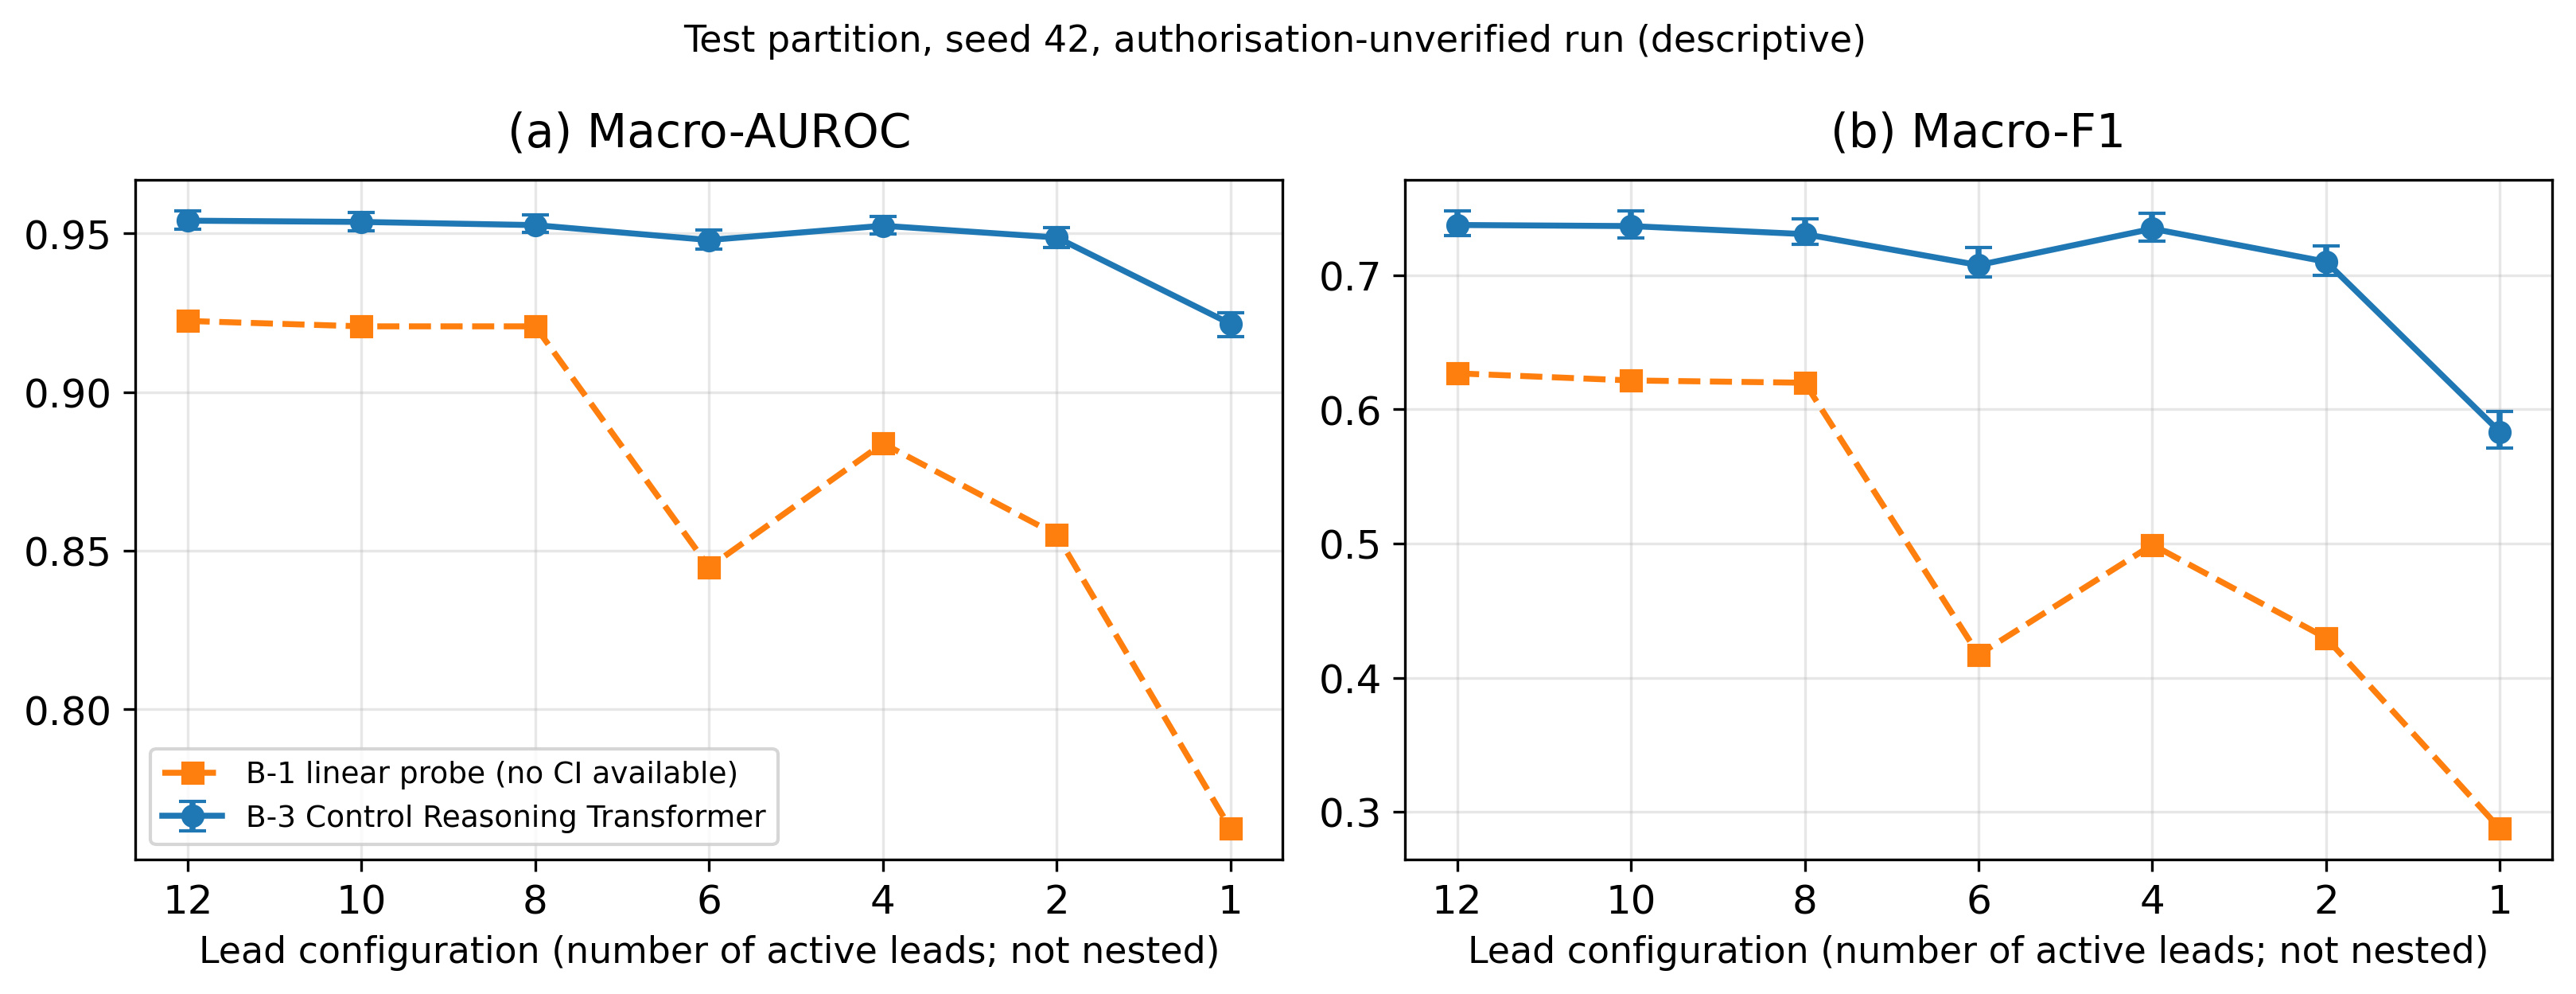
\includegraphics[width=\textwidth]{images/fig4_1_macro_metrics_by_configuration.jpg}
\caption{Test Macro-AUROC and Macro-F1 by Lead Configuration (B-3 with 95\% bootstrap intervals; B-1 point estimates only, since no intervals can be computed for it; drawn directly from the saved result files)}
\label{fig:ch4_1}
\end{figure}

Three features of the results stand out. First, removing the four derived limb leads changes almost nothing: from 12 to 10 to 8 leads, the macro-AUROC moves from 0.9540 to 0.9536 to 0.9526 and the macro-F1 from 0.7375 to 0.7367 to 0.7307, and the confidence intervals overlap. This is expected, because leads III, aVR, aVL and aVF are linear combinations of leads I and II (Section 3.3.5). The 10- and 8-lead configurations hide these leads from the model but remove no electrical information.

Second, performance does not fall steadily with the number of leads. The 4-lead configuration (macro-AUROC 0.9524, macro-F1 0.7347) is better than the 6-lead configuration (0.9479, 0.7076), and the 2-lead configuration (0.9487, 0.7101) is about as good as the 6-lead one. The configurations are not nested. The 6-lead configuration keeps all six limb leads but no chest lead, whereas the 4-lead and 2-lead configurations keep chest lead V1. The results therefore suggest that, for these eight conditions, V1 carries information that the full set of limb leads does not provide. This agrees with the observation that a well-chosen small lead subset can classify ECG abnormalities as well as larger sets \cite{LAI2021LEADSELECTION}. The lead-count ordering of the configurations is therefore not an ordering of information content. The difference between the 4- and 6-lead configurations (0.0045 in macro-AUROC and 0.0271 in macro-F1) is larger than the variation between seeds in either configuration on the validation partition (Table~\ref{tab:ch4_6}), and the macro-F1 intervals do not overlap, but no paired test of the difference is available.

Third, the single-lead configuration is clearly the weakest: its macro-AUROC is 0.9215 and its macro-F1 is 0.5832, against 0.9487 and 0.7101 for the 2-lead configuration. Section~\ref{sec:ch4_4_4} shows that this drop is concentrated in a few conditions.

The Diagnostic Failure Boundary of the protocol is defined from the ratio of each configuration's macro-F1 to the 12-lead macro-F1, with bootstrap intervals for that ratio. Those intervals are not implemented, so no Diagnostic Failure Boundary is reported, although the point estimates above show where macro-F1 falls most.

\subsection{Per-Condition Performance}\label{sec:ch4_4_4}

Table~\ref{tab:ch4_8} gives the per-condition F1 of the Control Reasoning Transformer on the test partition, and Figure~\ref{fig:ch4_2} shows the same values. The number of known labels and positives behind each condition is given in Table~\ref{tab:ch4_3}; these denominators are the same in every configuration.


\begin{table}[htbp]
\centering
\small
\setlength{\tabcolsep}{2pt}
\renewcommand{\arraystretch}{1.12}
\setstretch{1.0}
\caption[Test F1 per Condition]{Test F1 per Condition at Threshold 0.5 (Seed 42, Calibrated, Descriptive)}\label{tab:ch4_8}
\begin{tabular}{|c|c|c|c|c|c|c|c|}
\hline
\textbf{Condition} & \textbf{12} & \textbf{10} & \textbf{8} & \textbf{6} & \textbf{4} & \textbf{2} & \textbf{1} \\ \hline
NORM & 0.7778 & 0.7761 & 0.7732 & 0.7657 & 0.7701 & 0.7562 & 0.7310 \\ \hline
AFIB & 0.8028 & 0.7979 & 0.7966 & 0.7700 & 0.8036 & 0.7755 & 0.7479 \\ \hline
RBBB & 0.7855 & 0.7728 & 0.7363 & 0.6725 & 0.7785 & 0.7707 & 0.1266 \\ \hline
LBBB & 0.7910 & 0.7985 & 0.7955 & 0.7750 & 0.7821 & 0.7481 & 0.4565 \\ \hline
SBRAD & 0.8577 & 0.8599 & 0.8561 & 0.8593 & 0.8787 & 0.8539 & 0.8355 \\ \hline
STACH & 0.9121 & 0.9139 & 0.9165 & 0.9035 & 0.9121 & 0.9116 & 0.9058 \\ \hline
1AVB & 0.4230 & 0.4348 & 0.4315 & 0.4035 & 0.4410 & 0.3925 & 0.4172 \\ \hline
MI & 0.5500 & 0.5394 & 0.5395 & 0.5112 & 0.5116 & 0.4720 & 0.4451 \\ \hline
\end{tabular}
\end{table}

{\small Source: \path{runs/module4_v3/metrics/test_evaluation_summary.json}.}

\begin{figure}[htbp]
\centering
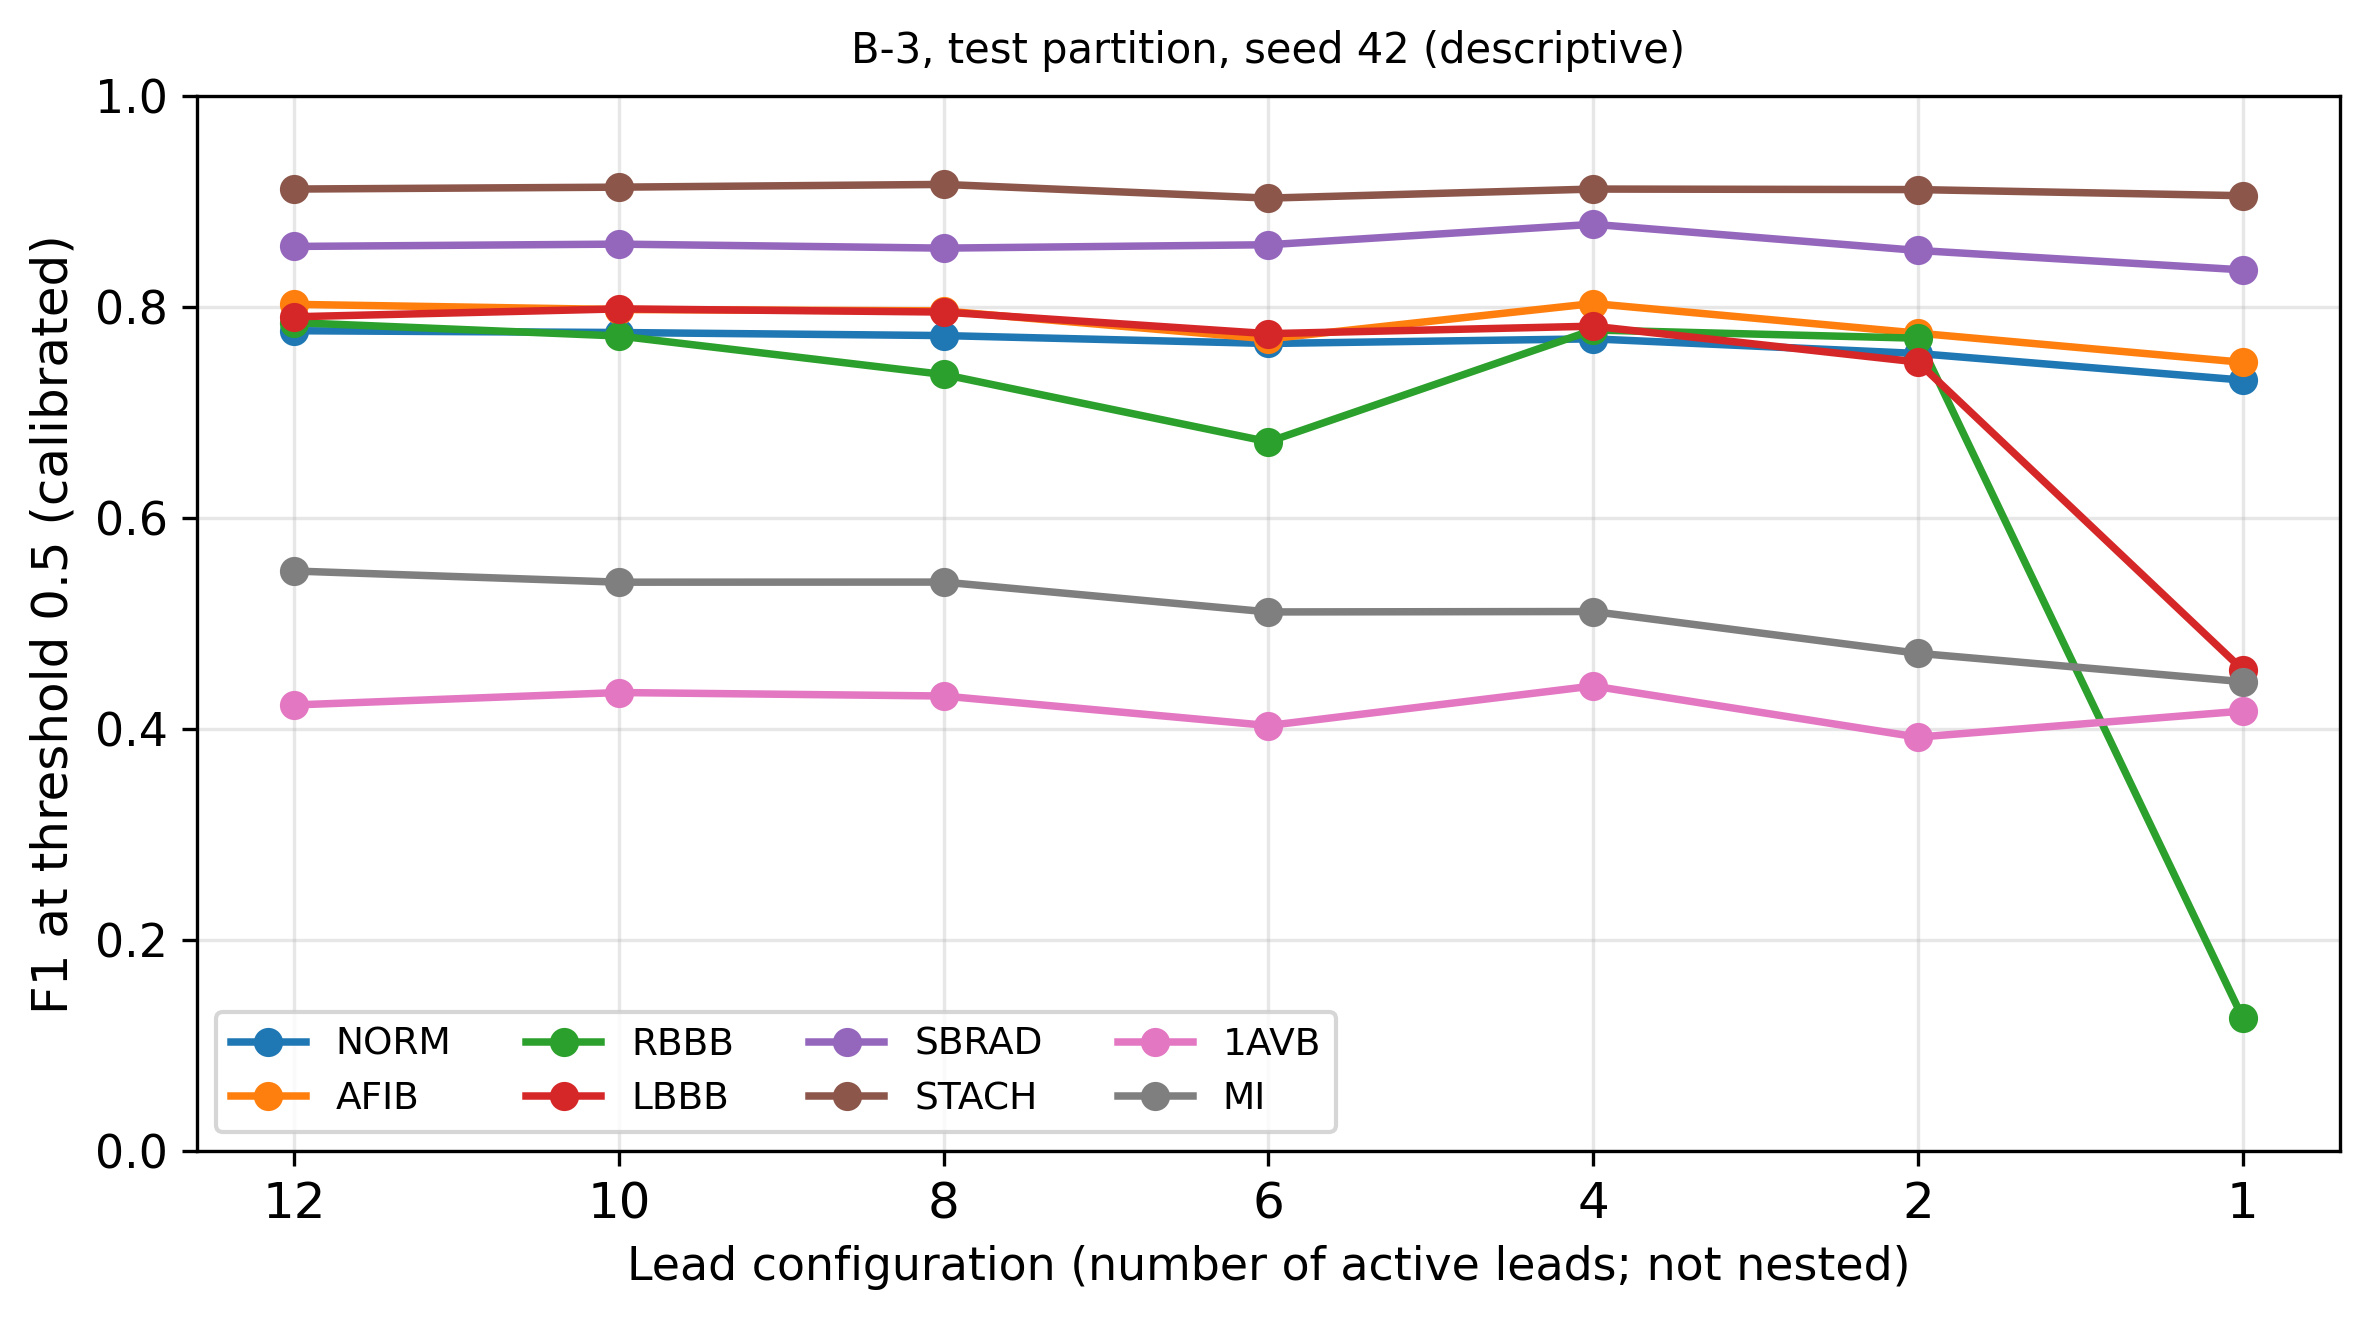
\includegraphics[width=\textwidth]{images/fig4_2_per_condition_f1.jpg}
\caption{Test F1 per Condition by Lead Configuration (B-3, seed 42; drawn directly from the saved test summary)}
\label{fig:ch4_2}
\end{figure}

The per-condition AUROC, from the same file, shows the same picture. Except for myocardial infarction, every condition kept an AUROC of at least 0.917 down to two leads; with lead II alone, the AUROC ranged from 0.8011 for myocardial infarction to 0.9940 for sinus tachycardia. The conditions fall into three groups.

\textbf{Rate-based conditions.} Sinus bradycardia and sinus tachycardia keep an AUROC of at least 0.982 and an F1 of at least 0.835 in every configuration, including the single-lead one. Both are defined mainly by heart rate, which can be measured from any lead that shows the QRS complexes. Lead II is retained in every configuration, so the heart rate measured from it, which reaches the model through the interval token, is the same in all seven (Section 3.3.7).

\textbf{Conduction blocks.} Right bundle branch block depends on chest lead V1 in a clear way. Its F1 is 0.7855 with all leads, falls to 0.6725 in the 6-lead configuration, which has no chest leads, recovers to 0.7785 and 0.7707 in the 4- and 2-lead configurations, which keep V1, and collapses to 0.1266 with lead II alone, where its recall is 0.074 and its AUROC 0.8408, against 0.9642 with all leads. Left bundle branch block degrades less: its F1 is between 0.748 and 0.799 down to two leads and falls to 0.4565 with one lead, where its AUROC is 0.9441. This pattern is consistent with the project schema, which assigns V1 and V6 to right bundle branch block (Table 3.2), but it does not show that the model uses those leads for the right reasons; establishing that is the purpose of the grounding gate.

\textbf{Low-F1 conditions.} First-degree atrioventricular block and myocardial infarction have the lowest F1 in every configuration. For first-degree atrioventricular block, the AUROC is high (0.9501 with all leads), but the F1 is only 0.4230, because the recall at threshold 0.5 is 0.32: only 149 test recordings receive a calibrated probability above 0.5 (92 true and 57 false positives), against 286 positive recordings. Myocardial infarction has the lowest AUROC (0.8475 with all leads, 0.8011 with one lead). Its criteria in the project schema depend on ST elevation or Q waves in contiguous leads of one territory (Table 3.2), Q waves are not among the extracted observations, and its labels come from three different labelling processes (Section~\ref{sec:ch4_1_1}).

\subsection{Performance by Cohort}\label{sec:ch4_4_5}

With all leads, the test macro-AUROC was 0.9476 for PTB-XL (4,358 recordings), 0.9509 for Chapman-Shaoxing (2,028) and 0.9379 for MIMIC-IV-ECG (989), and the corresponding macro-F1 values were 0.6767, 0.6775 and 0.7083. With lead II alone, the macro-AUROC was 0.9163, 0.9260 and 0.8981 (source: \texttt{dataset\_breakdown} field of the test summary).

The model performs at a similar level on all three cohorts, and the configuration pattern of Section~\ref{sec:ch4_4_3}, including the advantage of the 4-lead over the 6-lead configuration, appears in each of them (4-lead and 6-lead macro-AUROC: 0.9431 and 0.9406 for PTB-XL, 0.9618 and 0.9488 for Chapman-Shaoxing, 0.9367 and 0.9318 for MIMIC-IV-ECG). The macro-F1 of each cohort is lower than the macro-F1 of the pooled test partition. A likely reason is that some conditions have few positives in a single cohort, which lowers the cohort's per-condition F1; the project's post-evaluation audit records, for example, only 8 positive myocardial infarction recordings among the Chapman-Shaoxing test recordings. The MIMIC-IV-ECG results measure agreement with machine-generated statements rather than with clinicians, so they are not directly comparable with the other two cohorts \cite{REYNA2022ISSUES}. Because the three cohorts were pooled and split together, none of these results is an external validation on an unseen cohort. Nor are they comparable with published PTB-XL benchmarks \cite{STRODTHOFF2021PTBXL}, which use PTB-XL's own folds and label sets.

\subsection{Comparison Models}\label{sec:ch4_4_6}

The comparison models were evaluated on the same 7,375 test recordings and configurations (experiment E9). Table~\ref{tab:ch4_9} compares the linear probe (B-1) with the Control Reasoning Transformer (B-3).

{
\setlength{\tabcolsep}{2pt}
\renewcommand{\arraystretch}{1.12}
\begin{table}[htbp]
\centering
\footnotesize
\setstretch{1.0}
\caption[Linear Probe versus Control Reasoning Transformer]{Test Performance of the Linear Probe (B-1) and the Control Reasoning Transformer (B-3) (Descriptive)}\label{tab:ch4_9}
\begin{tabular}{|c|c|c|c|c|}
\hline
\textbf{Configuration} & \textbf{B-1 macro-AUROC} & \textbf{B-3 macro-AUROC} & \textbf{B-1 macro-F1} & \textbf{B-3 macro-F1} \\ \hline
12-lead & 0.9224 & 0.9540 & 0.6269 & 0.7375 \\ \hline
10-lead & 0.9207 & 0.9536 & 0.6216 & 0.7367 \\ \hline
8-lead & 0.9207 & 0.9526 & 0.6199 & 0.7307 \\ \hline
6-lead & 0.8448 & 0.9479 & 0.4172 & 0.7076 \\ \hline
4-lead & 0.8838 & 0.9524 & 0.4991 & 0.7347 \\ \hline
2-lead & 0.8550 & 0.9487 & 0.4296 & 0.7101 \\ \hline
1-lead & 0.7624 & 0.9215 & 0.2874 & 0.5832 \\ \hline
\end{tabular}
\end{table}
}

{\small Source: \path{runs/module4_v3/metrics/comprehensive_baseline_comparison.json}.}

The linear probe is a logistic regression for each condition, fitted on the frozen 12-lead representations of the training partition and applied without calibration at a threshold of 0.5. With all leads, it reaches a macro-AUROC of 0.9224, which shows that the frozen foundation-model representation already separates the eight conditions well. The Control Reasoning Transformer is higher in every configuration, by 0.03 in macro-AUROC and 0.11 in macro-F1 with 12, 10 or 8 leads, and by 0.24 to 0.30 in macro-F1 in the 6-, 4-, 2- and 1-lead configurations. The linear probe follows broadly the same pattern across configurations as the representation drift of Section~\ref{sec:ch4_4_7}: it is almost unchanged at 10 and 8 leads, falls most at 6 and 1 leads, and is better at 4 leads than at 6.

This comparison is descriptive. The two models differ at once in capacity, in training (the probe saw only 12-lead representations), in their observation and lead-availability inputs and in calibration, so the gap cannot be attributed to any one factor without ablations, which have not been run. The probe's per-recording predictions were not saved, so no paired intervals are available (Section~\ref{sec:ch4_3_2}).

The class-prevalence model (B-0) has a macro-AUROC of 0.5 and a macro-F1 of 0 by construction. The rule-engine model (B-2) is withdrawn as a comparison: it never predicts bundle branch block, because the extracted QRS duration never reaches 120 ms (Section~\ref{sec:ch4_4_8}), and the main branch of its atrial fibrillation rule never matches the extractor's label "Atrial Fibrillation / Irregular rhythm".

\subsection{Representation Stability}\label{sec:ch4_4_7}

Table~\ref{tab:ch4_10} gives the mean cosine similarity between the representation of each recording in a reduced configuration and its 12-lead representation, produced by the frozen foundation model (experiment E10).

\begin{table}[htbp]
\centering
\small
\setlength{\tabcolsep}{2pt}
\renewcommand{\arraystretch}{1.12}
\setstretch{1.0}
\caption{Mean Cosine Similarity to the 12-Lead Representation}\label{tab:ch4_10}
\begin{tabular}{|>{\raggedright\arraybackslash}p{0.15\textwidth}|>{\raggedright\arraybackslash}p{0.28\textwidth}|>{\raggedright\arraybackslash}p{0.23\textwidth}|>{\raggedright\arraybackslash}p{0.25\textwidth}|}
\hline
\textbf{Configuration} & \textbf{All partitions (36,888 recordings)} & \textbf{Test partition (7,375 recordings)} & \textbf{Standard deviation (all partitions)} \\ \hline
10-lead & 0.9981 & 0.9980 & 0.0021 \\ \hline
8-lead & 0.9971 & 0.9971 & 0.0027 \\ \hline
6-lead & 0.8775 & 0.8780 & 0.0621 \\ \hline
4-lead & 0.9041 & 0.9041 & 0.0520 \\ \hline
2-lead & 0.8762 & 0.8752 & 0.0621 \\ \hline
1-lead & 0.8144 & 0.8130 & 0.0849 \\ \hline
\end{tabular}
\par
{\small Source: \path{runs/module3_v1/reports/module3_cosine_similarity_summary.csv}.}
\end{table}

The representation changes very little when only derived leads are removed (similarity above 0.997) and changes most with a single lead (0.8144). Its ordering follows the classification results closely: the 4-lead representation stays closer to the 12-lead one than the 6-lead or 2-lead representations do, as the 4-lead classification results are better. The values measure the geometry of the representation, not diagnostic accuracy, and a lower similarity does not by itself mean lower accuracy, since the Control Reasoning Transformer was trained on the reduced representations as well.

Two cautions apply. Zero-masking changes the input distribution as well as the information available, and the two effects are hard to separate \cite{HOOKER2019ROAR}. In addition, ECG-FM is used outside its pretraining conditions (Section 3.3.6) \cite{MCKEEN2025ECGFM}, and record-level overlap between its pretraining data and the project's test recordings has not been checked.

\subsection{Clinical Observation Extractor}\label{sec:ch4_4_8}

The observation extractor was validated in a study of 250 MIMIC-IV-ECG recordings, sampled with seed 42 and compared with the measurements and statements produced by the dataset's automated interpretation program (\url{scripts/audit_clinical_observations.py}). The study was run on 6 October 2026, before the Module 4 freeze record was written on 15 October. The extractor source file was last modified on 23 September 2026, before the study, and its current SHA-256 hash matches the hash in the freeze record. The study therefore used the extractor code that was later frozen. The study did not record a code hash of its own.

Against the reference values, heart rate had a mean absolute error of 3.70 bpm (median 0.96 bpm; Pearson r = 0.866), the PR interval 21.57 ms (median 14.0 ms; r = 0.581) and the QRS duration 28.92 ms (median 26.0 ms; r = 0.255). Rhythm detection reached an F1 of 0.917 for sinus bradycardia, 0.681 for sinus tachycardia (sensitivity 0.517) and 0.475 for atrial fibrillation (sensitivity 0.633, precision 0.380, from 19 true and 31 false positives). The ST-segment and T-wave rules were not validated. The study labels the heart-rate measurement ``clinically validated'', although it compared it only with machine measurements (source: \texttt{reports/clinical\_observation\_validation.json}).



Heart rate, measured with the Pan–Tompkins-style detector of Section 3.3.7 \cite{PAN1985QRS}, agrees well with the machine measurements. The PR interval agrees only moderately, and the QRS duration agrees poorly. The reference values are themselves produced by an automated program, so the study measures agreement between two algorithms, not accuracy against a clinician; it is evidence of reasonableness rather than clinical validation.

The extracted observations of the training partition show two limitations directly. The extracted QRS duration of the 25,715 training recordings with a measurement lies between 50 and 110 ms, and none reaches 120 ms, because the QRS search window of ±60 ms at 100 Hz cannot measure a wider complex (Section 3.3.7). The PR interval lies between 100 and 250 ms, and 2,460 recordings exceed 200 ms. The rhythm labels written by the extractor are "Sinus rhythm" (13,673 recordings), "Sinus Bradycardia" (5,875), "Atrial Fibrillation / Irregular rhythm" (3,828), "Sinus Tachycardia" (2,239) and "Indeterminate rhythm" (210). Only "Sinus rhythm" matches the rhythm vocabulary of the context builder, so the other 12,152 training recordings (47.1\%) receive the same out-of-vocabulary rhythm token (Section 3.2).

The Control Reasoning Transformer therefore receives capped QRS values and a merged rhythm token, so the observation tokens cannot be assumed to contribute the information they were designed to provide. The same limits will matter more for the grounding gate: with the current extractor, a bundle branch block claim could never be supported by a measured QRS duration (Section 3.3.9).

\subsection{Discussion}\label{sec:ch4_4_9}

The first-half experiments establish a complete, reproducible classification pipeline across seven lead configurations and three cohorts. The frozen foundation model gives a representation that separates the eight conditions well (linear-probe macro-AUROC 0.9224 with all leads), and the Control Reasoning Transformer, trained once over all configurations, reaches a test macro-AUROC of 0.9540 with all leads and keeps it above 0.947 down to two leads. Diagnostic performance falls clearly only with a single lead, and it falls unevenly across conditions: rate-based conditions are unaffected, while right bundle branch block depends visibly on the presence of V1.

These findings answer only the diagnostic half of the research question. A model can keep a high AUROC on a single lead by relying on features that a cardiologist would not accept as evidence, and attention-based traces cannot settle this \cite{JAIN2019ATTENTION}; measuring it requires the grounding gate.

Several factors other than the reasoning model could explain parts of the results: the cohorts' different labelling processes, the encoder's non-native inputs and possible pretraining overlap, zero-masking, the observation extractor's limitations and the duplicated recordings. None of them invalidates the results as descriptive measurements, but together they limit how far the results can be generalised.

The test results are a single seed of a single authorisation-unverified run, and they should be confirmed by an authorised, separately versioned evaluation before any confirmatory claim is made. Section 4.3.1 lists the parts of the research programme for which no results exist yet. % IMPLEMENTATION
%-----------------------------------------
% Chapter 5 - Social Impact and Sustainability
%-----------------------------------------

\chapter{SOCIAL IMPACT \& SUSTAINABILITY}
\label{chap:ch5}

\section{SOCIAL IMPACT}\label{sec:ch5_1}

Most ECGs are interpreted automatically, and clinicians may accept computer statements without checking them \cite{SCHLAPFER2017COMPUTER}. Lower-cost devices that record fewer leads may widen access to cardiac care \cite{REYNA2022ISSUES}, and single-lead monitors are already used for rhythm assessment \cite{HANNUN2019CARDIOLOGIST}. A model developed on 12-lead recordings may therefore be applied to incomplete recordings without any warning that the evidence for some diagnoses is missing. This project studies that risk under controlled conditions, using seven zero-masked lead configurations and a frozen encoder. Its results show that the number of leads is a poor guide to reliability: the 4-lead configuration with V1 outperformed the 6-lead limb configuration, and the F1 score for right bundle branch block fell to 0.13 with lead II alone. Findings of this kind may help developers test models against stated lead configurations, and may in future help tell clinicians when an automated statement rests on leads that were not recorded.

These benefits are prospective. The project is a research evaluation, not a diagnostic tool, and it has not been clinically validated. Its test results are descriptive measurements from one seed of an authorisation-unverified run. The proposed grounding gate, with its SUPPORTED, CONTRADICTED and UNAVAILABLE states, and the Reasoning Failure Boundary have not been implemented, and the attention-based traces are not validated explanations \cite{GHASSEMI2021FALSEHOPE,JAIN2019ATTENTION}. The datasets are public PhysioNet releases whose de-identification is documented by their providers; the project adds no privacy measures of its own and claims no ethics approval or regulatory compliance. Because the cohorts were pooled, and the MIMIC-IV-ECG labels are machine-generated \cite{GOW2023MIMICIVECG}, the results are not an external validation.

\section{SUSTAINABILITY}\label{sec:ch5_2}

The project reuses the pretrained ECG-FM encoder, with 90,883,072 parameters, without retraining it \cite{MCKEEN2025ECGFM}. Only the Control Reasoning Transformer, with 1,830,657 parameters, was trained. The encoder's representations were computed once on the CPU for all 258,216 recording--configuration pairs and stored in about 0.83 GB, so the three training runs, of 5,763 to 5,973 seconds each, needed no passes through the encoder. A single model was trained for all seven configurations instead of one per configuration. Freeze records, split manifests and SHA-256 hashes made the Chapter 4 results checkable against their sources, although software versions and training logs were not recorded. No energy or carbon use was measured, so no savings are claimed. % CONCLUSION AND FUTURE WORK
%-----------------------------------------
% Chapter 6 - Conclusions and Future Work
%-----------------------------------------

\chapter{CONCLUSIONS AND FUTURE WORK}
\label{chap:ch6}

In conclusion, this project examined whether the diagnoses of an ECG foundation model remain supported by the evidence left after leads are removed. A frozen ECG-FM encoder \cite{MCKEEN2025ECGFM} and a Control Reasoning Transformer were evaluated on eight benchmark conditions across seven zero-masked lead configurations. The test macro-AUROC stayed between 0.9479 and 0.9540 down to two leads and fell to 0.9215 with lead II alone, and performance depended on which leads remained rather than how many.

These are descriptive results from one seed of an authorisation-unverified test run, and they do not establish clinical suitability or evidence grounding. The grounding gate, its metrics, the Reasoning Failure Boundary, the DFB and the AURDC are not yet implemented. The observation extractor cannot measure wide QRS complexes, morphology or Q waves, and lead removal is simulated rather than recorded.

As future work, the extractor and evidence schema will be repaired, the grounding gate implemented and the Reasoning Failure Boundary measured in an authorised, versioned evaluation. The SNOMED CT-based Clinical Knowledge Prior \cite{SNOMED2026CDSGUIDE} will then be added, and the system validated on independent cohorts.

\addtotoc{REFERENCES}
\begin{thebibliography}{99}

\bibitem{KLIGFIELD2007AHA}
P.~Kligfield \textit{et al.}, ``Recommendations for the Standardization and Interpretation of the Electrocardiogram: Part I: The Electrocardiogram and Its Technology,'' \textit{Circulation}, vol.~115, no.~10, pp.~1306--1324, 2007, doi:\url{https://doi.org/10.1161/CIRCULATIONAHA.106.180200}.

\bibitem{SURAWICZ2009AHA}
B.~Surawicz \textit{et al.}, ``AHA/ACCF/HRS Recommendations for the Standardization and Interpretation of the Electrocardiogram: Part III: Intraventricular Conduction Disturbances,'' \textit{Circulation}, vol.~119, no.~10, pp.~e235--e240, 2009, doi:\url{https://doi.org/10.1161/CIRCULATIONAHA.108.191095}.

\bibitem{WAGNER2009AHA}
G.~S.~Wagner \textit{et al.}, ``AHA/ACCF/HRS Recommendations for the Standardization and Interpretation of the Electrocardiogram: Part VI: Acute Ischemia/Infarction,'' \textit{Circulation}, vol.~119, no.~10, pp.~e262--e270, 2009, doi:\url{https://doi.org/10.1161/CIRCULATIONAHA.108.191098}.

\bibitem{SCHLAPFER2017COMPUTER}
J.~Schl\"apfer and H.~J.~Wellens, ``Computer-Interpreted Electrocardiograms,'' \textit{Journal of the American College of Cardiology}, vol.~70, no.~9, pp.~1183--1192, 2017, doi:\url{https://doi.org/10.1016/j.jacc.2017.07.723}.

\bibitem{HANNUN2019CARDIOLOGIST}
A.~Y.~Hannun \textit{et al.}, ``Cardiologist-level arrhythmia detection and classification in ambulatory electrocardiograms using a deep neural network,'' \textit{Nature Medicine}, vol.~25, no.~1, pp.~65--69, 2019, doi:\url{https://doi.org/10.1038/s41591-018-0268-3}.

\bibitem{STRODTHOFF2021PTBXL}
N.~Strodthoff, P.~Wagner, T.~Schaeffter, and W.~Samek, ``Deep Learning for ECG Analysis: Benchmarks and Insights from PTB-XL,'' \textit{IEEE Journal of Biomedical and Health Informatics}, vol.~25, no.~5, pp.~1519--1528, 2021, doi:\url{https://doi.org/10.1109/JBHI.2020.3022989}.

\bibitem{MCKEEN2025ECGFM}
K.~McKeen, S.~Masood, A.~Toma, B.~Rubin, and B.~Wang, ``ECG-FM: an open electrocardiogram foundation model,'' \textit{JAMIA Open}, vol.~8, no.~5, p.~ooaf122, 2025, doi:\url{https://doi.org/10.1093/jamiaopen/ooaf122}.

\bibitem{REYNA2022ISSUES}
M.~A.~Reyna \textit{et al.}, ``Issues in the automated classification of multilead ecgs using heterogeneous labels and populations,'' \textit{Physiological Measurement}, vol.~43, no.~8, p.~084001, 2022, doi:\url{https://doi.org/10.1088/1361-6579/ac79fd}.

\bibitem{OH2022LEADAGNOSTIC}
J.~Oh, H.~Chung, J.-M.~Kwon, D.-G.~Hong, and E.~Choi, ``Lead-agnostic Self-supervised Learning for Local and Global Representations of Electrocardiogram,'' in \textit{Proceedings of the Conference on Health, Inference, and Learning}, ser. \textit{Proceedings of Machine Learning Research}, vol.~174, 2022, pp.~338--353. [Online]. Available: \url{https://proceedings.mlr.press/v174/oh22a.html}.

\bibitem{LAI2021LEADSELECTION}
C.~Lai, S.~Zhou, and N.~A.~Trayanova, ``Optimal ECG-lead selection increases generalizability of deep learning on ECG abnormality classification,'' \textit{Philosophical Transactions of the Royal Society A: Mathematical, Physical and Engineering Sciences}, vol.~379, no.~2212, p.~20200258, 2021, doi:\url{https://doi.org/10.1098/rsta.2020.0258}.

\bibitem{PRESACAN2025RECON}
O.~Presacan \textit{et al.}, ``Evaluating the feasibility of 12-lead electrocardiogram reconstruction from limited leads using deep learning,'' \textit{Communications Medicine}, vol.~5, no.~1, p.~139, 2025, doi:\url{https://doi.org/10.1038/s43856-025-00814-w}.

\bibitem{GHASSEMI2021FALSEHOPE}
M.~Ghassemi, L.~Oakden-Rayner, and A.~L.~Beam, ``The false hope of current approaches to explainable artificial intelligence in health care,'' \textit{The Lancet Digital Health}, vol.~3, no.~11, pp.~e745--e750, 2021, doi:\url{https://doi.org/10.1016/S2589-7500(21)00208-9}.

\bibitem{JAIN2019ATTENTION}
S.~Jain and B.~C.~Wallace, ``Attention is not Explanation,'' in \textit{Proceedings of the 2019 Conference of the North American Chapter of the Association for Computational Linguistics: Human Language Technologies, Volume 1 (Long and Short Papers)}, 2019, pp.~3543--3556, doi:\url{https://doi.org/10.18653/v1/N19-1357}.

\bibitem{PAN1985QRS}
J.~Pan and W.~J.~Tompkins, ``A Real-Time QRS Detection Algorithm,'' \textit{IEEE Transactions on Biomedical Engineering}, vol.~BME-32, no.~3, pp.~230--236, 1985, doi:\url{https://doi.org/10.1109/TBME.1985.325532}.

\bibitem{SALIH2024XAICARDIO}
A.~M.~Salih \textit{et al.}, ``A review of evaluation approaches for explainable AI with applications in cardiology,'' \textit{Artificial Intelligence Review}, vol.~57, no.~9, p.~240, 2024, doi:\url{https://doi.org/10.1007/s10462-024-10852-w}.

\bibitem{SNOMED2026CDSGUIDE}
SNOMED International, ``SNOMED CT Clinical Decision Support Guide,'' \textit{SNOMED International documentation}, 2026. [Online]. Available: \url{https://docs.snomed.org/snomed-ct-practical-guides/snomed-ct-clinical-decision-support-guide} (accessed 19 Oct.~2026).

\bibitem{THORNE2018FEVER}
J.~Thorne, A.~Vlachos, C.~Christodoulopoulos, and A.~Mittal, ``FEVER: a Large-scale Dataset for Fact Extraction and VERification,'' in \textit{Proceedings of the 2018 Conference of the North American Chapter of the Association for Computational Linguistics: Human Language Technologies, Volume 1 (Long Papers)}, 2018, pp.~809--819, doi:\url{https://doi.org/10.18653/v1/N18-1074}.

\bibitem{WAGNER2020PTBXL}
P.~Wagner \textit{et al.}, ``PTB-XL, a large publicly available electrocardiography dataset,'' \textit{Scientific Data}, vol.~7, no.~1, p.~154, 2020, doi:\url{https://doi.org/10.1038/s41597-020-0495-6}.

\bibitem{LIU2025ARBITRARY}
C.~Liu, C.~Ouyang, Z.~Wan, H.~Wang, W.~Bai, and R.~Arcucci, ``Knowledge-enhanced Multimodal ECG Representation Learning with Arbitrary-Lead Inputs,'' in \textit{Findings of the Association for Computational Linguistics: EMNLP 2025}, 2025, pp.~7298--7316, doi:\url{https://doi.org/10.18653/v1/2025.findings-emnlp.385}.

\bibitem{HOOKER2019ROAR}
S.~Hooker, D.~Erhan, P.-J.~Kindermans, and B.~Kim, ``A Benchmark for Interpretability Methods in Deep Neural Networks,'' in \textit{Advances in Neural Information Processing Systems}, vol.~32, 2019. [Online]. Available: \url{https://papers.nips.cc/paper_files/paper/2019/hash/fe4b8556000d0f0cae99daa5c5c5a410-Abstract.html}.

\bibitem{VASWANI2017ATTENTION}
P.~Vaswani \textit{et al.}, ``Attention Is All You Need,'' in \textit{Advances in Neural Information Processing Systems}, vol.~30, 2017. [Online]. Available: \url{https://papers.nips.cc/paper_files/paper/2017/hash/3f5ee243547dee91fbd053c1c4a845aa-Abstract.html}.

\bibitem{WAGNER2022PTBXLDATA}
P.~Wagner, N.~Strodthoff, R.-D.~Bousseljot, W.~Samek, and T.~Schaeffter, ``PTB-XL, a large publicly available electrocardiography dataset (version 1.0.3),'' \textit{PhysioNet}, 2022, doi:\url{https://doi.org/10.13026/kfzx-aw45}.

\bibitem{ZHENG2020CHAPMAN}
J.~Zheng, J.~Zhang, S.~Danioko, H.~Yao, H.~Guo, and C.~Rakovski, ``A 12-lead electrocardiogram database for arrhythmia research covering more than 10,000 patients,'' \textit{Scientific Data}, vol.~7, no.~1, p.~48, 2020, doi:\url{https://doi.org/10.1038/s41597-020-0386-x}.

\bibitem{CINC2021DATA}
M.~Reyna \textit{et al.}, ``Will Two Do? Varying Dimensions in Electrocardiography: The PhysioNet/Computing in Cardiology Challenge 2021 (version 1.0.3),'' \textit{PhysioNet}, 2022, doi:\url{https://doi.org/10.13026/34va-7q14}.

\bibitem{GOW2023MIMICIVECG}
B.~Gow \textit{et al.}, ``MIMIC-IV-ECG: Diagnostic Electrocardiogram Matched Subset (version 1.0),'' \textit{PhysioNet}, 2023, doi:\url{https://doi.org/10.13026/4nqg-sb35}.

\bibitem{GUO2017CALIBRATION}
C.~Guo, G.~Pleiss, Y.~Sun, and K.~Q.~Weinberger, ``On Calibration of Modern Neural Networks,'' in \textit{Proceedings of the 34th International Conference on Machine Learning}, ser. \textit{Proceedings of Machine Learning Research}, vol.~70, 2017, pp.~1321--1330. [Online]. Available: \url{https://proceedings.mlr.press/v70/guo17a.html}.

\end{thebibliography}
 % REFERENCES

\end{spacing}
\end{document}
`
